%*****************************************************************
%** Thesis proyect: ''NAME''                                    **
%**                                                             **
%** by Alejandro Gómez-Conde                                    **
%** <alegzc@yahoo.com.mx>                                       **
%*****************************************************************

\documentclass[letterpaper,12pt,twoside,titlepage,onecolumn,openright,spanish]{book}
\usepackage{ucs}
\usepackage[utf8x]{inputenc}
\usepackage[T1]{fontenc}
\usepackage{graphicx}
\usepackage{subcaption}
\usepackage{rotating}
\usepackage{float}
\usepackage{url}
\usepackage{verbatim}
\usepackage{listings}
\usepackage{pdfpages}
\usepackage{amsmath}
\usepackage{fancyhdr}
\usepackage{natbib} % Referncias en formato APA
\usepackage[refpage,intoc,spanish]{nomencl} % Acrónimos
\usepackage[spanish]{babel}	% Titulos en español
\usepackage[spanish,linesnumbered,boxed,onelanguage]{algorithm2e}
\usepackage{lineno}
\SetAlCapSkip{1em}
% - - - - - - - - - - - - - - - - - - - - - - - - - - - - - - - - - -
%\usepackage[pdftex]{hyperref}
%\hypersetup{%
%   bookmarks=true%embedded system, partial reconfiguration, hardware function%
%}
% - - - - - - - - - - - - - - - - - - - - - - - - - - - - - - - - - -

\renewcommand{\nomname}{Acr\'onimos, abreviaturas y siglas}
%\makenomenclature
\renewcommand{\nompreamble}{En éste apartado se listan los acrónimos, abreviaturas y siglas usadas en éste texto. Se incluye una descripción breve, la respectiva traducción en los casos que así lo requieren entre paréntesis.
y la página donde aparece citada por primera vez a fin de que el lector pueda conocer el contexto en el que fue enunciada.}
%\nomenclature{c}{Speed of light in a vacuum inertial frame}
%\printnomenclature
%\renewcommand{\nompostamble}{findenomenclatura}
% - - - - - - - - - - - - - - - - - - - - - - - - - - - - - - - - - -
%\setlength{\parindent}{1.5cm}
%\setlength{\parskip}{}
%
% - - - - - - - - - - - - - - - - - - - - - - - - - - - - - - - - - -
% Abreviaturas personales (Inician por 'Z')
%\newcommand{\zxilinx}{\texttt{Xilinx}\textregistered}
%\newcommand{\zmicroblaze}{\texttt{MicroBlaze}\texttrademark}
%\newcommand{\cmd}[1]{\texttt{#1}}
% - - - - - - - - - - - - - - - - - - - - - - - - - - - - - - - - - -

% - - - - - - - - - - - - - - - - - - - - - - - - - - - - - - - - - -
%\author{Alejandro Gomez-Conde}
%\date{Dec 2011}

\begin{document}
\makenomenclature
%\nomenclature{c}{Speed of light in a vacuum inertial frame}
%\linenumbers %numerated lines in the document
%% - - - - - - - - - - - - - - - - - - - - - - - - - - - - - - - - - - - - -
% portada.tex-- Portada para tesis de posgrado de la Facultad de Ingeniería. UNAM.
% Realizada por Gengis Kanhg Toledo Ramírez (gengiskanhg.geo@yahoo.com)
% Basada en la portada escrita por: Tim Rohrer, LT, USN--31 July 1996 del NPS, Monterey, California. USA.
% y en el manual The Not So Short Introduction to LaTeX de Tobiaz Oetiker
% Eres libe de modificar este archivo de acuerdo a tus necesidades.
% 13 de Junio de 2007
% 
% Compile with:
% pdflatex portada.tex
% - - - - - - - - - - - - - - - - - - - - - - - - - - - - - - - - - - - - -
% Modificada por Julio Fernando Jimenez Vielma  CIC-IPN
% 2011
% - - - - - - - - - - - - - - - - - - - - - - - - - - - - - - - - - - - - -
% Adaptación para la maestría MCIC-CIC-IPN
% Alejandro Gómez <alegzc@yahoo.com.mx>
% 2012
% - - - - - - - - - - - - - - - - - - - - - - - - - - - - - - - - - - - - -
\documentclass{book}
%\usepackage[latin1]{inputenc} ¿used in Windows?
\usepackage[utf8]{inputenc} % Linux's text encoding scheme
\usepackage[spanish]{babel}
\usepackage{graphicx}

\setlength{\voffset}{-0.5cm}
\setlength{\hoffset}{0.7cm}
\setlength{\headsep}{0pt}
\setlength{\headheight}{0pt}
\setlength{\oddsidemargin}{-0.8in}
\setlength{\marginparwidth}{-0.5cm}
\setlength{\textwidth}{19.5cm}
\setlength{\footskip}{2pt}
\setlength{\topmargin}{0in}
\setlength{\textheight}{25cm}
\setlength{\fboxrule}{3pt}

\begin{document}
\thispagestyle{empty}

\begin{tabular}{p{3cm}p{15.0cm}}

\includegraphics[width=2.5cm]{fig/ipn.png}
\begin{center}
\rule[1cm]{1.5mm}{14.5cm}%vertical
\hspace{2pt}
\rule[0cm]{0.7mm}{15.5cm}%vertical
\hspace{2pt}
\rule[1cm]{1.5mm}{14.5cm}%vertical
\end{center}

\includegraphics[width=3cm]{fig/cic.png}
&
\vspace{-3.4cm}
\begin{center}
\Large{ \bf{INSTITUTO POLITÉCNICO NACIONAL}}
\\
\rule[0mm]{15.0cm}{0.35mm}%horizontal
\\
\rule[3mm]{15.0cm}{1.2mm}%horizontal
\\
\textbf{CENTRO DE INVESTIGACIÓN EN COMPUTACIÓN}

\vspace{2.8\baselineskip}

Laboratorio de Inteligencia Artificial \\
Laboratorio de Simulación y Modelado

\vspace{2.3\baselineskip}

{\Large \bf{Aprendizaje de fenómenos con representación\\ de estados en 2D}}

%\vfill
\vspace*{1.2cm}

\huge{\bf TESIS}

\vspace*{1.0cm}
{\large QUE PARA OBTENER EL GRADO DE:}

\vspace*{0.2cm}

\Large{\bf MAESTRO EN CIENCIAS DE LA COMPUTACIÓN}

%\vspace*{0.2cm}
%\large{MEC�NICA - DISE�O MEC�NICO}

\vspace*{0.2cm}
P R E S E N T A:

\vspace*{1.0cm} {\Large \bf{Ing. Héctor Daniel Moreno Leyva}}

\vspace*{1.0cm}
Directores de tesis:

\large{\bf Dr. Salvador Godoy Calderón\\M. C. Germán Téllez Castillo}

\vspace*{1.8cm}
\Large{México, CDMX}\hspace*{5cm}\Large{Octubre 2020}

\end{center}

\end{tabular}

%\end{center}
\newpage % La razón de esta página en blanco es la de mantener el orden (izq, derecha)
%          en el resto del documento al que se adjuntará...
\thispagestyle{empty}
$ $ % junk
\end{document}
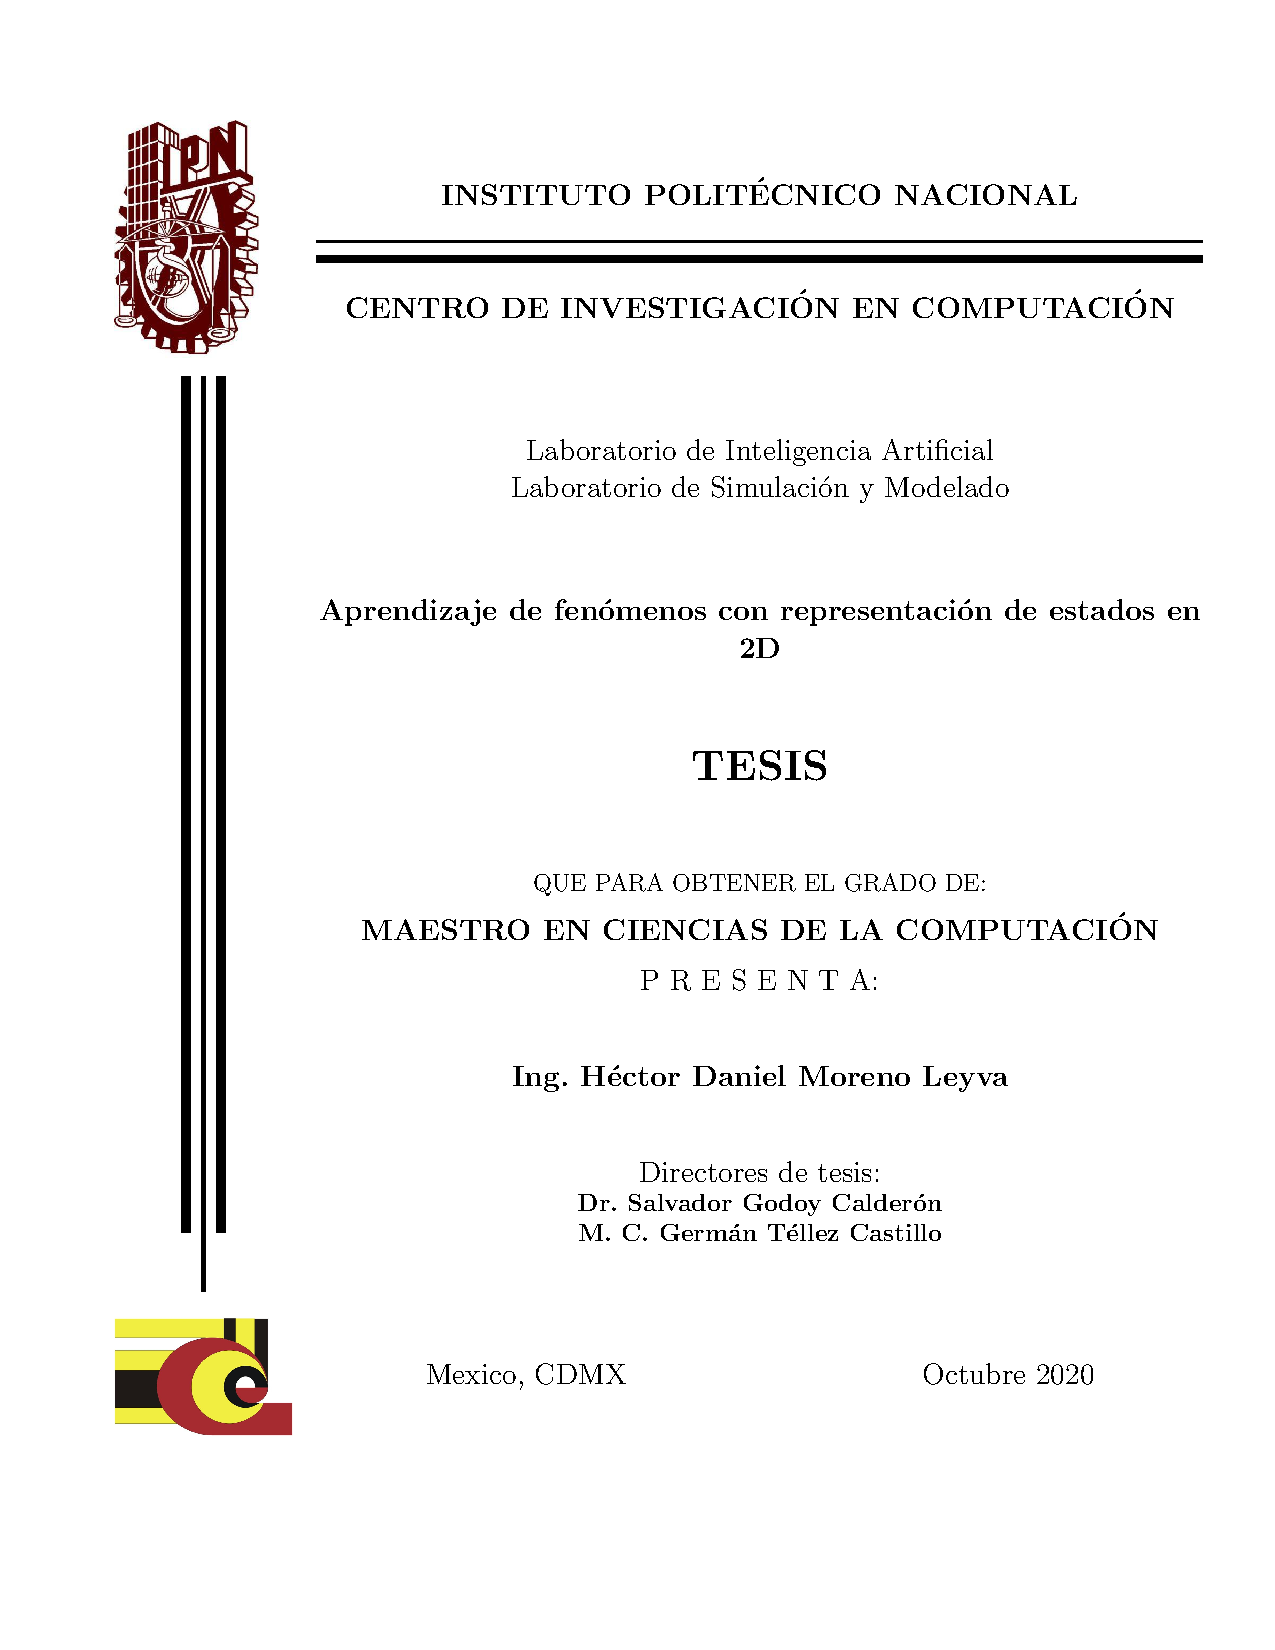
\includepdf{../portada/portada.pdf}
%\include{cesion_derechos} % Carta de cesión de derechos para publicación

% + + + + + + + + + + + + + + + + + + + + + + + + + + + + + + + + + +
% + + + + + + + + + + + + + + + + + + + + + + + + + + + + + + + + + +
% +          _             _                           _            +
% +   __ _  | |__    ___  | |_   _ __    __ _    ___  | |_          +
% +  / _` | | '_ \  / __| | __| | '__|  / _` |  / __| | __|         +
% + | (_| | | |_) | \__ \ | |_  | |    | (_| | | (__  | |_          +
% +  \__,_| |_.__/  |___/  \__| |_|     \__,_|  \___|  \__|         +
% +                                                                 +
% + + + + + + + + + + + + + + + + + + + + + + + + + + + + + + + + + +
% + + + + + + + + + + + + + + + + + + + + + + + + + + + + + + + + + + 
\pagestyle{plain}
\pagenumbering{roman}
\cleardoublepage
\chapter*{Resumen}
\addcontentsline{toc}{chapter}{Resumen}
\bigskip
\noindent Para la modelación de sistemas físicos, químicos y biológicos, los autómatas celulares han sido una herramienta importante por su capacidad de modelar sistemas dinámicos de manera discreta en el espacio y tiempo; y a su vez también ha sido una herramienta cuyo uso es limitado por la complejidad que existe en la generación de las reglas de evolución que modela el sistema completamente. Se ha demostrado que los algoritmos de aprendizaje simbólicos y sub-simbólicos han resultado de gran utilidad para generar modelos interpretables a partir de un conjunto de datos, es por esto que en el presente trabajo se busca estudiar cómo es posible facilitar el uso de estas herramientas de modelado realizando un propuesta de algoritmo de aprendizaje automático que nos permita generar reglas a partir de un conjunto de datos representativos obtenidos de cierto fenómeno, sin perder la semántica que se encuentra embebida en los datos de los que se está aprendiendo.

% + + + + + + + + + + + + + + + + + + + + + + + + + + + + + + + + + +
% + + + + + + + + + + + + + + + + + + + + + + + + + + + + + + + + + +
%\vspace*{1cm}
\bigskip
\bigskip
%\cleardoublepage
\chapter*{Abstract}
\addcontentsline{toc}{chapter}{Abstract}
\bigskip
The modelation of physical, biological and chemistry systems, the cellular automata models have been an important tool for their capacity to model dynamical systems in a discrete way in space and time; also it is a tool whose use is limited by the complexity that exists to select the right evolve transition rules to model the system completely. It has been demonstrated that symbolic and sub-symbolic algorithms of learning have been of great utility to generate interpretative models from a dataset, is because of this that in order to facilitate the use of this tools, we are proposing a model that let us generate a set of rules from a representative dataset of a certain phenomena, without loosing the semantics of what does the data represent.
  % to be generated
%
\cleardoublepage
\chapter*{Summary}
\addcontentsline{toc}{chapter}{Summary}
\noindent
This thesis has the following organization.
\begin{description}
% Introducción
% \item[Chapter 1] It begins with an introduction to Embedded Systems (E.S.), it sets up 
% 
% it sets up the context theory so that other students can replicate this proyect.
% 
% the theory context so that a reader can understand the concepts. It also discusses the history of the area, defines the characteristics of such a resolve, it argues the importance of research, presents the objectives of the thesis and concludes with the hypothesis that will solve the problem.

% Introducción
\item[Chapter 1] begins with ...

% Fundamento teórico
\item[Chapter 2] has ....

%Desarrollo e Implementación
\item[Chapter 3] describes ...

% Pruebas y resultados
\item[Chapter 4] presents ...

\item[Chapter 5] Collect all results to ....

\end{description}% Fin de la descripción de la organización del documento   
\chapter*{THANKS}\label{agrad}
\markboth{THANKS}{}

\baselineskip 1em
%\thispagestyle{empty}

Here go the thanks.

    % to be completed
%% + + + + + + + + + + + + + + + + + + + + + + + + + + + + + + + + + +
% Índice de acrónimos, abreviaturas y siglas
\cleardoublepage
\thispagestyle{headings}
\markboth{\nomname}{\nomname}
\addcontentsline{toc}{chapter}{\nomname}
\makenomenclature
\printnomenclature %[1.5cm]
%\addcontentsline{toc}{chapter}{\nomname}

  
% # # # # # # # # # # Falta agregar sus entradas al índice general # # # # # # # # # #
\pagebreak
%\cleardoublepage
\tableofcontents % Índice general

%\clearpage
%\listoffigures % Lista de figuras
%\addcontentsline{toc}{chapter}{\'Indice de figuras}

%\clearpage
%\pagebreak
%\listoftables % Lista de tablas
%\addcontentsline{toc}{chapter}{\'Indice de tablas}

%\clearpage
%\pagebreak
%\lstlistoflistings % Lista de tablas	
%\addcontentsline{toc}{chapter}{\'Indice de listados}


 
%\printnomenclature
\pagebreak  % Fin de numeración romana
\cleardoublepage
\pagestyle{headings}
\pagenumbering{arabic}

\chapter{Introducción}
%
Desde hace ya varios siglos los seres humanos se han beneficiado de la modelación y simulación de sistemas dinámicos para entender la naturaleza. En la actualidad existe una amplia gama de métodos de simulación y modelado;  uno de ellos son los autómatas celulares. 

Los autómatas celulares son sistemas dinámicos en el que el espacio y el tiempo son discretos. Los estados de las células de una lattice regular, son
actualizados en base a reglas de evolución de interacción local.Las reglas de evolución local son obtenidas en base a la experiencia, experimentos, o análisis de la información del problema de tal forma que las restricciones del problema se cumplan.

Hoy en día este problema ya está siendo investigado desde distintos aspectos, sin embargo muchos de ellos se centran en crear métodos específicos para el área de estudio en el que se está realizando la modelación del fenómeno, por ejemplo, la búsqueda de reglas para modelar la conversión de un área rural a un área urbana, o la búsqueda de reglas para modelar patrones de bioconvección en algas unicelulares; y otros trabajos de propósito más general que emplean algoritmos evolutivos para la generación de reglas donde el comportamiento específico no es conocido, esto es, llegar de un estado inicial a un estado final sin tomar en cuenta lo que suceda en los estados intermedios.
Este último trabajo es el más apegado a lo que se busca en esta tesis, sin embargo, un punto importante en el que se diferencian los dos trabajos es que a nosotros nos interesa tomar en cuenta la información del fenómeno de principio a fin, para crear un conjunto de reglas que repliquen este fenómeno lo más preciso posible, esto es, pasando por cada uno los estados de los que tenemos información.

\section{Definiciones}

\subsection{Autómata celular}


Los autómatas celulares son sistemas dinámicos y discretos en espacio, estado y tiempo. Propuestos por los matemáticos John von Neumann y Stanislaw Ulam como un sistema discreto para crear un modelo reduccionista de la auto-replicación, creando así en 1950 el primer autómata celular como método para calcular el movimiento de un líquido. 
\\
En 1970 el autómata celular “Game of Life” inventado por John Conway \citep{gardner1970mathematical}, que consiste de dos dimensiones y dos estados, se volvió ampliamente conocido, sobre todo en la comunidad computacional.
\\
En 1981 Stephen Wolfram empezó a trabajar independientemente en autómatas celulares, en 1985 conjeturo que la regla 110 de un autómata celular elemental era equivalente a una máquina de Turing, cosa que demostró Matthew Cook en el 2004 \citep{cook2004universality}.
\\
Como podemos ver a través de los años con el incremento de poder de cómputo y el trabajo que se ha ido realizando alrededor de los autómatas celulares, ha ido incrementado el interés por utilizarlos para modelar sistemas naturales y artificiales.
\\
Los autómatas celulares pueden ser empleados como una alternativa a las ecuaciones diferenciales para modelar sistemas físicos \citep{toffoli1984cellular}, y como un modelo de cómputo paralelo y distribuido \citep{hillis1984connection}.
\\
\\
El uso exitoso de los autómatas celulares en distintos campos, tales como:

\begin{itemize}
	\item Simulación de tránsito \citep{simon1998simplified}
	\item Dinámica de fluidos  \citep{margolus1986cellular}
	\item Formación de patrones \citep{tamayo1987cellular,boerlijstk}
	\item Conexiones con los lenguajes formales \citep{nordahl1989formal,culik1990computation}
	\item Modelación y simulación de diversos sistemas físicos \citep{vichniac1984simulating,manneville2012cellular} y biológicos \citep{ermentrout1993cellular}
\end{itemize}

es una de las razones por las cuales este trabajo de tesis es de importancia.
\\
\\
La mayoría de los autómatas celulares poseen las siguientes cinco características\citep{ilachinski2001cellular}:

\begin{itemize}
	\item{\textbf{Una lattice de células discretas}: El sistema consiste de una estructura llamada lattice la cual puede ser de dimensionalidad  $\mathnormal{d}$, donde $\mathnormal{d\; \epsilon\; \aleph\cup\{0\}}$}
	\item{\textbf{Homogeneidad}: Todas las células son equivalentes.}
	\item{\textbf{Estados discretos}: Cada célula toma un estado de un conjunto finito de estados discretos.}
	\item{\textbf{Interacciones locales}: Cada célula interactúa solo con las células que están en su vecindad.}
	\item{\textbf{Sistemas dinámicos discretos}: En cada paso de tiempo discreto, cada célula actualiza su estado actual de acuerdo a una función o regla de evolución que toma como entrada los estados de las células vecinas y da como salida un estado del conjunto de estados.}
\end{itemize}

\textbf{Definición 1.1.1} Un autómata celular es una 5-tupla $\mathnormal{(L, D, S, H, f)}$ donde:
\begin{itemize}
	\item $\mathnormal{L}$ es una matriz de dimensión $\mathnormal{d}$
	\item $\mathnormal{D\; \epsilon\; \aleph\cup\{0\}}$ y es la dimensión del autómata.
	\item $\mathnormal{S}$ es un conjunto finito de elementos llamados estados y es denotado por:
	\\
	$\mathnormal{S=\{s_{k}:k \epsilon \{0,\dots,|S|-1\}\}}$, donde $\mathnormal{|S|}$ es la cardinalidad del conjunto de estados $S$
	\item $H$ es un subconjunto finito de $Z^{d}$ llamado vecindad y es denotado por $\{v_{j}:x_{1,j},\dots,x_{d,j}:j\epsilon1,\dots,|H|\}$, donde los elementos $v_{j}$ son llamados vectores vecindad.
	\item $f$ es una función de $S^{|H|}$ en $S$, llamada la función de evolución o regla.
\end{itemize}
\textbf{Definición 1.1.2} En un autómata celular se dice que posee fronteras nulas, si el vecino de la izquierda (o de la derecha) de la célula del extremo izquierdo (o derecho) se considera siempre como cero.
\\
\\
\textbf{Definición 1.1.3} En un autómata celular se dice que posee fronteras periódicas, si los extremos derecho
e izquierdo son adyacente el uno del otro.

\subsection{Aprendizaje automático}

El área de aprendizaje automático es un sub-area de la Inteligencia Artificial (AI), que se basa en distintos enfoques para mejorar en el desempeño de un programa computacional sobre una tarea utilizando la experiencia que se tiene sobre la tarea. El aprendizaje puede ser de distintos tipos, los principales siendo: aprendizaje supervisado, aprendizaje no supervisado y aprendizaje reforzado.
\\
\\
\textbf{Aprendizaje supervisado}: Consiste en el uso de un conjunto de entrenamiento para mejorar el desempeño en el programa computacional utilizando como entrada pares $(x,y)$ y la tarea es encontrar una funcion $f$ que al ingresar $x$ produzca $y$ como salida. 
\\
\\
\textbf{Aprendizaje no supervisado}: Consiste en el uso de un conjunto de entrenamiento donde se conocen valores de entrada $x$, pero estos datos no están etiquetados. La tarea entonces es encontrar una función $f$ tal, que al ingresar $x$ como entrada produzca como salida $y$ de tal forma que $y$ sea igual para todas las entradas $x$ que compartan cierta medida de similitud.
\\
\\
\textbf{Aprendizaje reforzado}: En este tipo de aprendizaje no tenemos conocimiento previo sobre la tarea, si no que se va obteniendo experiencia sobre la tarea como se va realizando, y se va ajustando nuestro programa computacional con respecto a la métrica de desempeño obtenida sobre la tarea en cada iteración.

\subsection{Algoritmos genéticos}

Los algoritmos genéticos son algoritmos de búsqueda basados en las mecánicas de la selección natural. Combinan el supervivencia del mas apto con el intercambio de información para formar un algoritmo de búsqueda con el novedoso instinto de búsqueda humana.  


\section{Planteamiento del problema}

Dada una secuencia de estados bidimensionales, encontrar un conjunto de reglas que al ingresarlas a un autómata celular puedan reproducir estos estados.

\section{Objetivos}
%Esta sección describe el objetivo general y los objetívos específicos de esta tesis.
%
\subsection{Objetivo general}
\noindent \paragraph{Diseñar un nuevo (simbólico o sub-simbólico) algoritmo de aprendizaje para aprender reglas que gobiernan un fenómeno para las cuales nosotros solo tenemos como entrada rejillas estados en 2 dimensiones.}

\subsection{Objetivos específicos}
\begin{itemize}
\item Revisar y seleccionar algunos algoritmos de aprendizaje de reglas para el problema planteado.
\item Proponer un nuevo algoritmo de aprendizaje.
\item Diseñar procedimientos específicos para la simplificación de locales a globales de los conjuntos de reglas.
\item Construir el modelo de autómata celular que reproduce el fenómeno cuando es alimentado con las reglas aprendidas.
\item Usar errores de aprendizaje y generalización para evaluar los resultados de cada experimento. 
\end{itemize}

\section{Justificación}
La búsqueda de reglas para que un autómata celular pueda reproducir un fenómeno es compleja debido a que el espacio de búsqueda crece exponencialmente tomando en cuenta la cardinalidad del vecindario y la cardinalidad del espacio de estados. Es por esto que se requiere una búsqueda que pueda mejorar el desempeño en este espacio de búsqueda tomando en consideración información adicional.

\subsection{Beneficios esperados}
Esta tesis pretende generar una propuesta de algoritmo genético multi-poblacional distribuido el cual pueda solucionar el problema planteado.

\subsection{Alcances y límites}
En este trabajo se pretende encontrar un algoritmo que pueda aprender un fenómeno del cual solo se cuenta con un conjunto de estados 2-dimensional las reglas de evolución para que al ingresarlas a un autómata celular pueda replicar el fenómeno completo, para esto utilizamos los estados obtenidos de la evolución de autómatas celulares, ya que obtener estados de la forma requerida de fenómenos reales era una tarea ardua, la cual no se pudo realizar con los recursos de tiempo que se tenían disponibles.

\nomenclature{AC}{Autómata celular}
\ % Introducción 
% CAP 2
\chapter{Marco teórico}

\section{Autómata celular}
Los autómatas celulares son sistemas dinámicos y discretos en espacio, estado y tiempo. Propuestos por los matemáticos John von Neumann y Stanislaw Marcin Ulam como un sistema discreto para crear un modelo reduccionista de la auto-replicación, creando así en 1950 el primer autómata celular como método para calcular el movimiento de un líquido \citep{biaynicki2012}. 
\\

En 1970, John Horton Coway inventó un autómata celular llamado “Game of life” \citep{gardner1970mathematical}, el cual es un autómata celular de dos dimensiones y dos estados, y que se hizo popular a partir de su publicación (octubre de 1970) en la columna: Mathematical Games de Martin Gardner en la revista Scientific American.
\\

En 1984, Stephen Wolfram clasifica a los autómatas celulares lineales en cuatro clases \citep{WOLFRAM19841}. Y en 1985 conjeturó que la regla 110 de un autómata celular elemental era equivalente a una máquina de Turing, cosa que demostró Matthew Cook en el 2004 \citep{cook2004universality}.
\\

Como podemos ver, a través de los años con el incremento del poder de cómputo y del trabajo que se ha ido realizando alrededor de los autómatas celulares, también ha ido en aumento el interés por utilizarlos para modelar sistemas naturales y artificiales.
\\

Los autómatas celulares pueden ser empleados como una alternativa a las ecuaciones diferenciales para modelar sistemas físicos \citep{toffoli1984cellular}, y como un modelo de cómputo paralelo y distribuido \citep{hillis1984connection}.
\\

Los autómatas celulares han sido aplicados exitosamente en diferentes áreas del conocimiento, tales como: la simulación de tránsito \citep{nagel1992cellular,simon1998simplified}, la dinámica de fluidos  \citep{margolus1986cellular} y la formación de patrones \citep{tamayo1987cellular,boerlijstk}. Asimismo, se ha tenido éxito en las conexiones con los lenguajes formales \citep{nordahl1989formal,culik1990computation} y, como se mencionó anteriormente, en el modelado y simulación de diversos sistemas físicos \citep{vichniac1984simulating,manneville2012cellular} y biológicos \citep{ermentrout1993cellular}.
\\

Como podemos observar, los autómatas celulares tienen un gran alcance en la resolución de diversos problemas.
\\

Los autómatas celulares clásicos poseen las siguientes cinco características \citep{ilachinski2001cellular}:

\begin{itemize}
	\item{\textbf{Una lattice de células discretas}: El sistema consiste de una estructura llamada lattice la cual puede ser de dimensionalidad  $\mathnormal{d}$, donde ${d\; \epsilon\; N\cup\{0\}}$}
	\item{\textbf{Homogeneidad}: Todas las células son equivalentes.}
	\item{\textbf{Estados discretos}: Cada célula toma un estado de un conjunto finito de estados discretos.}
	\item{\textbf{Interacciones locales}: Cada célula interactúa sólo con las células que están en su vecindad.}
	\item{\textbf{Sistemas dinámicos discretos}: En cada paso de tiempo discreto, cada célula actualiza su estado actual de acuerdo a una función o regla de evolución que toma como entrada los estados de las células vecinas y da como salida un estado del conjunto de estados.}
\end{itemize}

\section{Algoritmos genéticos}

Los algoritmos genéticos fueron desarrollados por John Holland, sus colegas y estudiantes en la Universidad de Michigan. Los objetivos de esta investigación fueron los que se enlistan a continuación \citep{goldberg_2012}.
\begin{enumerate}
	\item Abstraer y explicar rigurosamente los procesos adaptativos de los sistemas naturales.
	\item Diseñar sistemas artificiales de software que retuvieran los mecanismos importantes de los sistemas naturales.
\end{enumerate}

El tema central de la investigación sobre los algoritmos genéticos ha sido la robustez, el balance entre la eficiencia y la eficacia necesaria para sobrevivir en distintos ambientes. Los algoritmos genéticos han probado teórica y experimentalmente que proveen una búsqueda robusta en espacios complejos.
\\

La implementación de un algoritmo genético consta de la definición de:

\begin{itemize}
	\item La representación de las soluciones.
	\item La función de aptitud.
	\item Los operadores de selección, mutación y cruza.
	\item El tamaño de la población.
	\item Los valores de probabilidad con la que se aplican los operadores genéticos.
\end{itemize}

El pseudocódigo del Algoritmo 1, ilustra el funcionamiento de un algoritmo genético simple.
\\

\begin{algorithm}[h] 
	
	\SetAlgoLined
	Inicializar la población con candidatos aleatorios de la solución\;
	Evaluar cada candidato\;
	\While{La condicion de paro no se satisfaga}{
		\textbf{Paso 1:} Seleccionar a los padres\;
		\textbf{Paso 2:} Recombinar los pares de padres\;
		\textbf{Paso 3:} Mutar a los hijos\;
		\textbf{Paso 4:} Evaluar a los nuevos candidatos\;
		\textbf{Paso 5:} Seleccionar a los individuos para la siguiente generación\;
	}
	
	\caption{Pseudocódigo de un algoritmo genético simple.}
\end{algorithm}


A continuación, se explican de manera general los requerimientos de los algoritmos genéticos y posteriormente, en la sección \ref{Ga-Nuggets} y en la sección \ref{LRDEA}, se precisan detalles para cada algoritmo genético implementado en este trabajo de investigación.

\subsection{Representación}

Este paso consiste en crear un vínculo entre el contexto original del problema y espacio de solución del problema, donde la evolución se lleva a cabo. Esto se realiza definiendo cómo es que las soluciones serán especificadas y guardadas para que puedan ser manipuladas por una computadora.
\\

Los objetos que forman posibles soluciones en el contexto original, son llamados fenotipos; mientras que su codificación en el espacio de solución se denominan genotipos.

\subsection{Función de aptitud}

El rol de la función de aptitud es representar los requerimientos a los que se debe adaptar la población. Desde la perspectiva de resolución de problemas, representa la tarea a ser resuelta en el contexto evolutivo.
\\

Técnicamente  es una función o procedimiento que le asigna una medida cualitativa a los genotipos.

\subsection{Población}

La población forma la unidad básica de evolución, los individuos son objetos estáticos que no cambian o se adaptan, es la población la que lo hace. La diversidad de la población es la que indica las diferentes soluciones que hay presentes.

\subsection{Mecanismo de selección de padres}

Este mecanismo tiene como objetivo distinguir a los mejores individuos para que sean los padres de la siguiente generación, con base en su calidad. Este mecanismo, junto con el mecanismo de selección de sobrevivientes, son los responsables de generar mejoras en la calidad de las soluciones.

\subsection{Recombinación}

Este operador es un operador variacional que recombina la información de dos padres en uno o más genotipos descendientes. La recombinación es una operación estocástica, esto significa que cómo se eligen los genes de los padres y cómo se combinan, depende del azar.
\\

El principio detrás de la recombinación es sencillo --- al aparear a dos individuos con diferentes pero deseables atributos, se puede obtener una descendencia que combine ambas características. 

\subsection{Mutación}

Este operador variacional unario, cuando es aplicado a un genotipo, resulta en un mutante ligeramente modificado. El operador de mutación siempre es un operador aleatorio y es el causante de ingresar ''sangre fresca'' a la población.

\subsection{Mecanismo de selección de sobrevivientes}

Este mecanismo toma la decisión de qué individuos serán los elegidos para pasar a la siguiente población; esta decisión se basa frecuentemente en sus valores de aptitud. Al contrario del mecanismo de selección de padres, que es aleatorio, este mecanismo es frecuentemente determinista. 

\section{GA-Nuggets}
\label{Ga-Nuggets}

El GA-Nuggets (\textit{Genetic Algorithm Nuggets}), fue diseñado por \cite{book_data_mining} para el modelado de dependencias en dos versiones: la primera versión es de una población centralizada de individuos, donde diferentes individuos pueden representar reglas de predicción para diferentes atributos objetivo. La segunda versión mantiene una población distribuida de muchas sub-poblaciones, donde cada una de ellas evoluciona de manera independiente, pero con la posibilidad de que algunos individuos puedan migrar entre las sub-poblaciones. En esta segunda versión, cada población tiene asociado un atributo objetivo a predecir, es por esto que todos los individuos de cada sub-población representan reglas para predecir el mismo atributo objetivo.

\subsection{Representación de los individuos}

Cada individuo representa una regla de predicción candidata de la forma IF $Ant$ THEN $Cons$, donde $Ant$ es el antecedente de la regla y $Cons$ es el consecuente.
\\

El antecedente $Ant$ consiste en una conjunción de condiciones, donde cada condición es un par atributo-valor de la forma $A_i = V_{ij}$, donde $A_i$ es el i-ésimo atributo y $V_{ij}$ es el j-ésimo valor del atributo $A_i$.
\\

Es importante mencionar que el algoritmo solo maneja valores categóricos, por lo que es necesario discretizar los valores.
\\

El consecuente $Cons$ consiste en un solo par atributo-valor de la forma $G_k = V_{kl}$, donde $G_k$ es el k-ésimo atributo objetivo y $V_{kl}$ es el l-ésimo valor del atributo $G_k$. El conjunto de atributos objetivos son seleccionados por el usuario entre todos los atributos del conjunto de datos y el resto de los atributos se utiliza como atributos predictivos.
\\

Un individuo es codificado en una cadena de longitud fija conteniendo $z$ genes, donde $z$ es el número de atributos considerando los atributos predictivos y objetivo.
\\

De los valores de los atributos codificados en el genoma, solo un subconjunto de los valores de los atributos sera decodificado. Para realizar esto, se utiliza un valor que no se encuentre entre los posibles valores de los atributos, por ejemplo $-1$, para indicar que ese gen no sera decodificado en un antecedente para la regla; gracias a esto, a pesar de que la longitud de la cadena sea fija, podemos tener un antecedente de longitud variable.
\\

Una vez que se generó el antecedente de la regla, el algoritmo selecciona el atributo objetivo que incremente la aptitud del individuo.

\subsection{Función de aptitud}

La función de aptitud cuyo dominio es entre $0$ y $1$, consiste de dos partes: la primera mide el grado de interés de la regla, y la segunda mide su certeza de predicción. El grado de interés de la regla se define en dos términos, el primero se refiere al antecedente y el segundo al consecuente de la regla.
\\

El grado de interés de la regla se evalúa con una métrica de teoría de la información, donde el grado de interés para el antecedente de la regla está dado por:

\begin{equation} 
\label{eq:1}
AntInt = 1- \left( \frac{\sum\limits_{i=1}^n InfoGain(A_i)/n}
{log_2(\left| dom(G_k) \right|)}
\right),
\end{equation}

\noindent
donde $n$ es el número de atributos que ocurren en el antecedente de la regla y $|dom(G_k)|$ es la cardinalidad del dominio (es decir, el número de valores posibles) del atributo de destino $G_k$ que se produce en el consecuente. El término $log$ se incluye en la fórmula \ref{eq:1} para normalizar el valor de $AntInt$, de modo que esta medida tenga un valor entre $0$ y $1$. El $InfoGain$ viene dado por:

\begin{equation} \label{eq:2}
InfoGain(A_i)=Info(G_k)-Info(\left.G_k\right| A_i),
\end{equation}
donde,

\begin{equation}  \label{eq:3}
Info(G_i)=-\sum\limits_{i=1}^{mk}\left(Pr(V_{kl}) log_2 (Pr(V_{kl}))\right),
\end{equation}
y

\begin{equation} \label{eq:4}
Info(\left. G_k \right| A_i)=\sum\limits_{i=1}^{n_i}\left( Pr(V_{ij})\left(-\sum\limits_{j=1}^{mk} Pr\begin{pmatrix}V_{kl}|V_{ij}\end{pmatrix} log_2 \begin{pmatrix}Pr\begin{pmatrix}V_{kl}|V_{ij}\end{pmatrix}\end{pmatrix}\right)  \right).
\end{equation}


Donde $m_k$ es el número de posibles valores que puede tomar el atributo objetivo $G_k$, $n_i$ es el número de posibles valores para el atributo $A_i$, $Pr(X)$ denota la probabilidad de $X$ y $Pr(X|Y)$ denota la probabilidad de $X$ dado $Y$.
\\

La métrica que proporciona $AntInt$ puede ser justificada porque, en general, dado un atributo predictor $A_i$, cuya ganancia de información sea alta con respecto a $G_k$, nos lleva a considerar que $A_i$ es un buen predictor de $G_k$ cuando se considera individualmente, ignorando sus interacciones con otros atributos predictivos.
\\

Por lo anterior, si se considera que el usuario ya conoce los atributos que son buenos predictores del atributo objetivo $G_k$, estos atributos podrían no parecerle interesantes al usuario.
\\

Adicionalmente, a los atributos que tienen baja ganancia de información y que aparecen en el antecedente de la regla, el usuario podría considerarlos como irrelevantes por sí solos, sin embargo, cuando interaccionan con los otros atributos podrían generar que éstos aumenten su relevancia, lo que los haría interesantes para el usuario.
\\

La computación del grado de interés del consecuente de la regla está basada en la idea de que mientras más raro sea el valor de un atributo objetivo con respecto a un valor común del atributo, más interesante será para el usuario. En otras palabras, mientras mas grande sea la frecuencia relativa en el conjunto de entrenamiento del valor predicho en el consecuente, menos interesante será para el usuario.
\\

Puntualmente, la regla para predecir el grado de interés del consecuente de la regla es:

\begin{equation} \label{eq:5}
ConsInt= (1-Pr(G_{kl}))^{1/\beta},
\end{equation}

\noindent
donde $Pr(G_{kl})$ es la frecuencia relativa del valor del atributo objetivo $G_{kl}$, y $\beta$ es un parámetro especificado por el usuario.
\\

La segunda parte de la función de aptitud mide la exactitud predictiva de la regla, y está dada por:

\begin{equation} \label{eq:6}
PredAcc= \frac{|A\&C|-1/2}{|A|},
\end{equation}

\noindent
donde $|A\&C|$ es el número de ejemplos que satisfacen tanto el antecedente como el consecuente de la regla, y $|A|$ es el número de ejemplos que satisfacen solo el antecedente. El término $1/2$ es para penalizar las reglas que cubren pocos ejemplos de entrenamiento.
\\

Finalmente, la función de aptitud sería:
\begin{equation} \label{eq:7}
Fitness= \frac{w_1(AntInt+ConsInt)/2+w_2PredAcc}{w_1+w_2},
\end{equation}

\noindent
cuyo dominio estaria entre $0$ y $1$, y donde $w_1$ y $w_2$ son pesos definidos por el usuario, con valores positivos mayores a $0$.

\subsection{Método de selección y operadores genéticos}

GA-Nuggets utiliza el bien conocido ''selección por torneo'' con un tamaño de torneo de 2, y utiliza una cruza uniforme extendida con un procedimiento de reparación. En la cruza uniforme existe una probabilidad de aplicar cruza a dos individuos y otra probabilidad para intercambiar cada gen. Después de que se realiza la cruza, el algoritmo verifica si se generó un individuo inválido. Si es así, se inicia un procedimiento de reparación para generar individuos validos. El operador de mutación transforma de forma aleatoria el valor de un atributo en otro, dentro del mismo dominio del atributo.
\\

Además de la cruza y la mutación, se agregan otros dos operadores: insertar-condición y eliminar-condición, que controlan el tamaño de las reglas que están siendo evolucionadas, de la siguiente forma: mientras mayor sea el número de condiciones en el antecedente de la regla actual, menor será la probabilidad de aplicar el operador insertar-condición; y este operador no se aplicará si el antecedente ya tiene el máximo número de condiciones especificado por el usuario. En cambio, la probabilidad de aplicar el operador eliminar-condición será mayor mientras menor sea el número de condiciones en el antecedente de la regla; y este operador no se aplicará si el antecedente solo tiene una condición.

\section{Enfoque OCAT (One Clause At a Time)}

El enfoque ''Una Cláusula A la Vez'' u OCAT, por sus siglas en inglés (One Clause At a Time) es un enfoque que trata de resolver dos debilidades con las técnicas de aprendizaje bayesianas y conexionistas como lo son las redes neuronales, estas debilidades son las siguientes:

\begin{enumerate}
	\item Las formas en que estos métodos funcionan y producen recomendaciones pueden no ser atractivos por los expertos en el dominio. 
	\item El conjunto de entrenamiento puede no contener suficientes ejemplos como para que garanticen resultados estadisticamente significantes. Como resultado estos métodos pueden no ser fidedignos para aplicaciones reales. 
\end{enumerate}

Este enfoque está basado en conceptos de lógica matemática y optimización discreta. El enfoque es de naturaleza \emph{avara}, en el sentido de que busca aceptar a todos los ejemplos positivos y rechazar tantos ejemplos negativos como sea posible. Esto se realiza sucesivamente para cada una de las cláusulas que genera, hasta que ya no tenga más ejemplos negativos para rechazar.
\\

El enfoque OCAT busca generar un conjunto de cláusulas que pueden estar en forma normal conjuntiva (FNC) o forma normal disyuntiva (FND). Es conocido \citep{peysakh1987fast} que cualquier función Booleana puede ser transformada en forma FNC o FND. 
\\

Algunas suposiciones que este enfoque toma son las siguientes:

\begin{itemize}
	\item Se tienen observaciones que describen el comportamiento del sistema a aprender.
	\item Que un conjunto de $n$ atributos de estas observaciones describen totalmente el sistema.
	\item Cada una de las observaciones pertenece a una y solo una de las K clases.
	\item Que las observaciones están libres de ruido.
	\item También asume que la clase a la que pertenece la observación es la correcta. 
\end{itemize}

El siguiente pseudocódigo ejemplifica el funcionamiento general del enfoque OCAT.
\\
\begin{algorithm}[H] 
	\SetAlgoLined
	$i = 0; C=\emptyset;$\{Inicializaciones\}\;
	\While{$E^- \neq \emptyset $}{
		\textbf{Paso 1:} $i \leftarrow i+1$\;
		\textbf{Paso 2:} Encontrar una cláusula $c_i$ que acepte todos los miembros de $E^+$ mientras rechaza tantos miembros sea posible de $E^-$\;
		\textbf{Paso 3:} Sea$ E^-(c_i)$ el conjunto de miembros de $E^-$ que son rechazados por $c_i$\;
		\textbf{Paso 4:} Sea $ C \leftarrow C \land c_i$\;
		\textbf{Paso 5:} Sea $ E^- \leftarrow E^- - E^- (c_i)$\;
	}
	
	\caption{Pseudocódigo de enfoque OCAT para generar cláusulas en forma normal conjuntiva.}
\end{algorithm}

\subsection{Heurística RA1}
El enfoque heurístico, denominado RA1 por \textit{Randomized Algorithm 1}, fue propuesto en \citep{DESHPANDE199875} y es un algoritmo que selecciona de forma aleatoria dentro los mejores atributos candidatos, tal cual se muestra en el algoritmo \ref{algorithmra1}. De esta manera se evita el estancamiento del algoritmo en un mínimo local. 
\\

\textbf{Definiciones:}

\begin{itemize}
	\item $C$ es el conjunto de atributos en la clausula actual.
	\item $A_k$ es un atributo dado que $A_k\in A$, donde $A$ es el conjunto de todos los atributos $A_1,\dots,A_k$
	\item $POS(A_k)$ el numero total de ejemplos positivos en $E^+$ que serán aceptados si el atributo $A_k$ es incluido en la clausula actual.
	\item $NEG(A_k)$ el numero total de ejemplos negativos en $E^-$ que serán aceptados si el atributo $A_k$ es incluido en la clausula actual. 
	\item $l$ el tamaño de la lista de candidatos.
	\item $ITRS$ el numero de veces que el procedimiento de formación de clausulas es repetido.
\end{itemize}

\begin{algorithm}[H] %or another one check
	
	\SetAlgoLined
	\SetKwFor{While}{mientras}{hacer}{}
	Hacer por $ITRS$ numero de iteraciones\;
	\While{$E^-\not = \emptyset$}{
		$C=\emptyset$ (inicialización);
		\SetKwFor{While}{mientras}{hacer}{fin}
		\While{$E^+\not = \emptyset$}{
				 \textbf{Paso 1:} Clasificar en orden descendente todos los atributos $a_i \in a$ (donde $a_i$ es $A_i$ o $\neg A_i$) de acuerdo a su valor $POS(a_i)/NEG(a_i)$. Si $NEG(a_i)=0$, entonces $POS(a_i)/NEG(_i)=1000$ (i.e., un valor arbitrariamente alto)\;
				 \textbf{Paso 2:} Formar una lista de candidatos de los atributos que tienen los $l$ valores más altos $POS(a_i)/NEG(a_i)$\;
				 \textbf{Paso 3:} Elegir al azar un atributo $a_k$ de la lista de candidatos\;
				 \textbf{Paso 4:} Sea $C \leftarrow C \vee a_k$ el conjunto de atributos en la cláusula actual\;
				 \textbf{Paso 5:} Sea $E^+(a_k)$ el conjunto de miembros de $E^+$ aceptados cuando $a_k$ se incluye en la cláusula FNC actual\;
				 \textbf{Paso 6:} Sea $E+ \leftarrow E^+-E^+(a_k)$\;
				 \textbf{Paso 7:} Sea $a \leftarrow a-a_k$\;
				 \textbf{Paso 8:} Calcular los nuevos valores $POS(a_i)$ para todos $a_i \in a$\;
				 
				}
		}
				 
	\end{algorithm}
			
		
	\begin{algorithm}[h]
	\LinesNumbered
	\setcounter{AlgoLine}{9}
	\SetAlgoLined
	\SetKwBlock{Begin}{}{fin}
	\Begin{
				 
			\textbf{Paso 9:} Sea $E^-(C)$ el conjunto de miembros de $E^-$ que son rechazados por $C$\;
			\textbf{Paso 10:} Sea $E^- \leftarrow E^- - E^-(C)$\;
			\textbf{Paso 11:} Reiniciar $E^+$\;
	
	}
	\textbf{elegir} el sistema Booleano final que tenga el menor número de cláusulas, de los sistemas ITRS anteriores.
	\caption{La heurística RA1 \citep{DESHPANDE199875}} \label{algorithmra1}
\end{algorithm}
\newpage
\section{Algoritmo Quine–McCluskey}

Este algoritmo es un método utilizado para la simplificación de funciones Booleanas y fue desarrollado por Willard V.Quine 1955 y extendido por Edward J. McCluskey en 1956. Este método involucra dos pasos:
\begin{enumerate}
	\item Encontrar los implicantes primos de la función.
	\item Usar esos implicantes primos para encontrar los implicantes primos esenciales de la función, así como los otros implicantes primos necesarios para realizar la cobertura de la función.
\end{enumerate}

El pseudocódigo a continuación define este algoritmo, que es empleado en la metodología de experimentación para minimizar el conjunto de cláusulas que se obtienen a partir de los 

\begin{algorithm}
	\SetAlgoLined
	\SetKwBlock{Begin}{inicio}{}
	\Begin{
		\SetKwBlock{Begin}{inicio}{fin}
	Organizar los términos mínimos en orden ascendente\;
	Formar como máximo $n+1$ grupos en función del número de unos presentes en sus representaciones binarias\footnotemark \;
	

}
\end{algorithm}


\begin{algorithm}
	  \LinesNumbered
	\setcounter{AlgoLine}{13}

\SetAlgoLined
\SetKwBlock{Begin}{}{fin}
\Begin{
	\SetKwBlock{Begin}{inicio}{fin}
	\Begin{
		Obtener los implicantes primos:
		
		\While{no se tengan todos los implicantes primos}{
			comparar los términos mínimos presentes en grupos sucesivos  
			\newline
			\If{existe un cambio en la posición de un solo bit}{
				Tomar ese par de dos términos mínimos\;
				Colocar el símbolo ''\textunderscore'' en la posición del bit de cambio\;
				Mantener el resto de los bits tal como están\;
				
	}}}
	\Begin{
		Formular la tabla de primos implicantes, que consiste en un conjunto de filas y columnas:
		\newline
		\Begin{
			Los implicantes primos se colocan en sentido de las filas\;
			Los términos mínimos se colocan en sentido de las columnas\;
			Colocar un $''1''$ en las celdas correspondientes a los términos mínimos que se cubren en cada implicante primo\;
		}
	}
	\Begin{Encontrar los implicantes primos esenciales:
		\newline
	\ForAll{término mínimo de la función Booleana}{
		observar cada columna de la tabla de primos implicantes 
		\newline
		\If{el término mínimo está cubierto solo por un implicante primo}{
			este término es un implicante esencial y formará parte de la función Booleana simplificada
		}
		eliminar la fila de cada implicante primo esencial y las columnas correspondientes a los términos mínimos que están cubiertos en ese implicante primo esencial
	}
	}
	}
	
	\caption{Método Tabular Quine-McCluskey: para simplificar funciones Booleanas.}
\end{algorithm}

\footnotetext{Para $n$ variables Booleanas en una función Booleana, o para $n$ bits en su equivalente binario de términos mínimos.} 

\nomenclature{FND}{Forma Normal Disyuntiva}
\nomenclature{RA1}{Randomized Algorithm 1}
\nomenclature{GA-Nuggets}{Genetic Algorithm- Nuggets}
\nomenclature{OCAT}{One Clause At a Time} % Marco teórico
\chapter{Estado del Arte}

De los trabajos que existen en la actualidad, podemos mencionar tres que resultan de especial interés para este trabajo de investigación. Las tres metodologías de nuestro interés son las siguientes:
\begin{itemize}
	\item Búsqueda de reglas locales para un autómata celular mediante el análisis estadístico de las observaciones de un fenómeno.
	\item Configuración de reglas locales para un autómata celular mediante el empleo de algoritmos evolutivos.
	\item Búsqueda de reglas locales para un autómata celular mediante el empleo de algoritmos evolutivos para satisfacer un patrón especifico.
\end{itemize}

Estos son algunos de los enfoques para emplear los autómatas celulares como herramienta para modelar fenómenos, que si bien tienen relación con este trabajo de tesis, no se conectan directamente con el.

\section{Cellular Automata Automatically Constructed from a Bioconvection Pattern}

Esta investigación \citep{kawaharada2016cellular} se centra en descubrir reglas de evolución para un autómata celular unidimensional, empleando métodos de análisis estadísticos para determinar dichas reglas, a partir de los datos observados de los patrones de bioconvección que son generados como resultado de la respuesta a la estimulación luminosa de un tipo de alga unicelular llamada \emph{Euglena gracilis}.
\\
El experimento consistió en iluminar por la parte de abajo de un contenedor anular conteniendo una suspensión de E. gracilis con una fuerte intensidad de luz. Los individuos, al ser alcanzados por la luz, sufren de fototaxis negativa, lo cual provoca que se acumulen cerca de la superficie.

Como la densidad del E. gracilis es mas pesada que el agua, las regiones ricas en esta alga se precipitan al fondo para conducir el flujo local. Estas interacciones entre los individuos y el flujo eventualmente forma patrones de bioconvección.
\\
El proceso se realizó de la siguiente forma:

\begin{enumerate}
	\item Recopilación de imágenes de los patrones de bioconvección.
	\item Transformación de las imágenes recopiladas a escala de grises.
	\item Uso de filtros para la eliminación del ruido.
	\item Discretización de las imágenes en escala de grises.
	\item Se predetermina el número de estados para el sitio $k$ y se discretiza la información observada acorde a esto.
	\item Basado en el número de vecinos establecido $m$ se calcula la frecuencia con la que aparecen los estados por cada combinación de posibles estados vecinos.
	\item Con base en esta frecuencia se determinan las reglas locales para el AC.
\end{enumerate}

\section{Discovery of Transition Rules for Cellular Automata Using Artificial Bee Colony and Particle Swarm Optimization Algorithms in Urban Growth Modeling}

En este trabajo \citep{naghibi2016discovery} se muestra un método para descubrir las reglas de transición de un autómata celular de lattice bidimensional que modele el crecimiento urbano empleando un algoritmo de optimización de colonia de abejas artificiales. Para ello, se utilizan como datos de entrada información multitemporal sensada remotamente de el área urbana de la ciudad de Urmia, Irán.
\\
El autómata celular en este trabajo se define con la siguiente ecuación:

\begin{equation} \label{eq:8}
P^t_{ij} = S^t_{ij}\times\Omega^t_{ij}\times Con\times e_r,
\end{equation}

donde:
\begin{itemize}
	\item $P^t_{ij} $ es el potencial de desarrollo de una celda $ij$.
	\item $S^t_{ij}$ es la idoneidad de la celda $ij$ para cambiar basada en factores relevantes en el tiempo $t$.
	\item $\Omega^t_{ij}$ es el efecto que tiene la densidad de desarrollo del vecindario.
	\item $Con$ es una condición funcional que se vuelve verdadero cuando se encuentra la idoneidad de la celda.
	\item $e_r$ es un termino para la perturbación estocástica por errores.
\end{itemize}

El potencial de desarrollo se compara con un valor umbral para determinar si una célula no urbanizada va a poder ser transformada en una célula urbanizada en el tiempo $t+1$. Entonces, los valores a encontrar son los valores de umbral para los cuales se produce la transición de una célula no urbanizada a una urbanizada.
\\
Como requerimiento para la evaluación del algoritmo, se emplean otras dos técnicas además de la colonia de abejas artificiales,las cuales son:
\begin{itemize}
	\item Particle Swarm Optimization (PSO)
	\item Logistic Regression
\end{itemize}

Los siguientes diagramas de continuación muestran el procedimiento que se siguió con cada uno de los algoritmos para la calibración de las reglas para el autómata celular.

\begin{figure}[H]
	\centering
	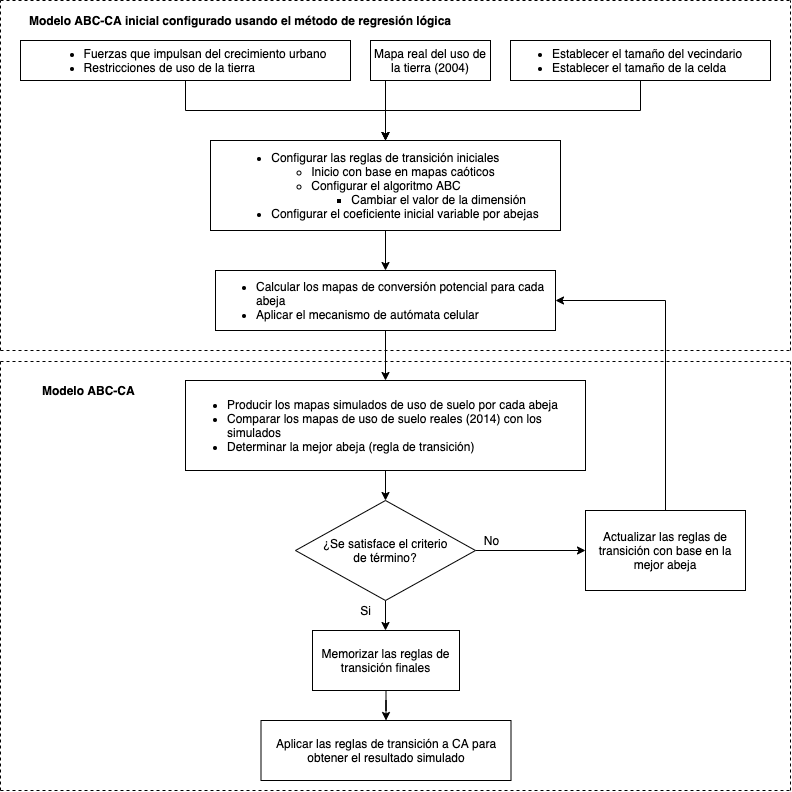
\includegraphics[width=\linewidth]{fig/abejas}
	\caption{Modelo para la obtención de reglas del autómata celular empleando un algoritmo de optimización de colonia de abejas artificiales.}
	\label{fig:abc}
\end{figure}

\begin{figure}[H]
	\centering
	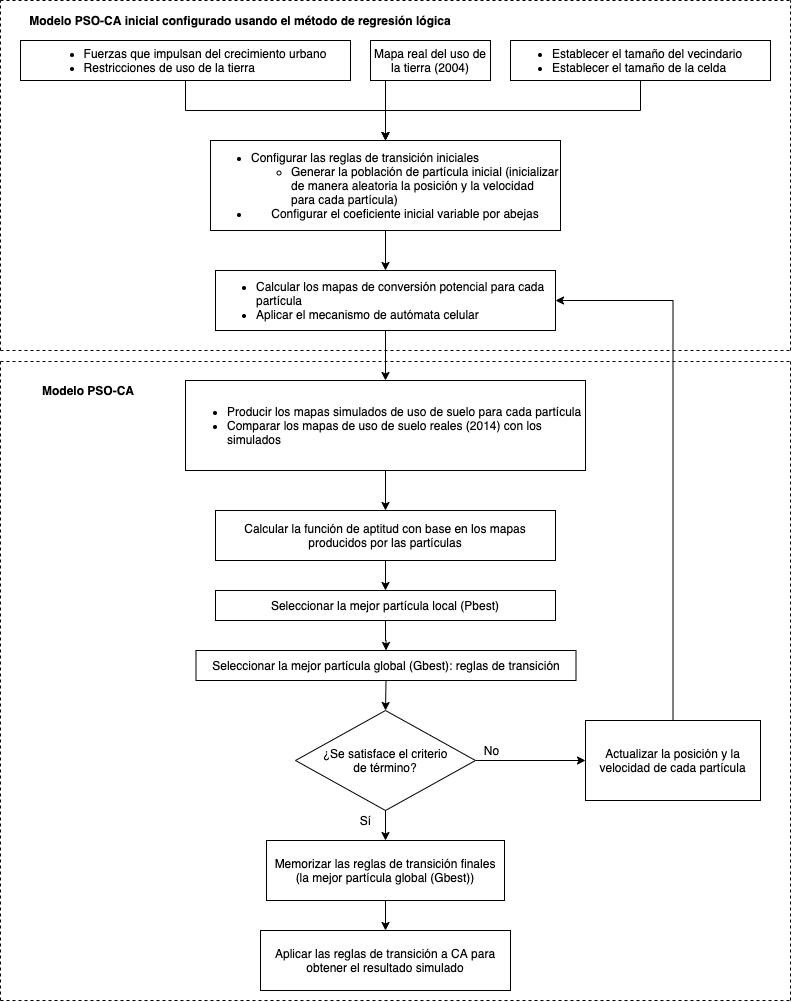
\includegraphics[width=\linewidth]{fig/particulas}
	\caption{Modelo para la obtención de reglas del autómata celular empleando un algoritmo de optimización de enjambre de partículas.}
	\label{fig:pso}
\end{figure}

\begin{figure}[H]
	\centering
	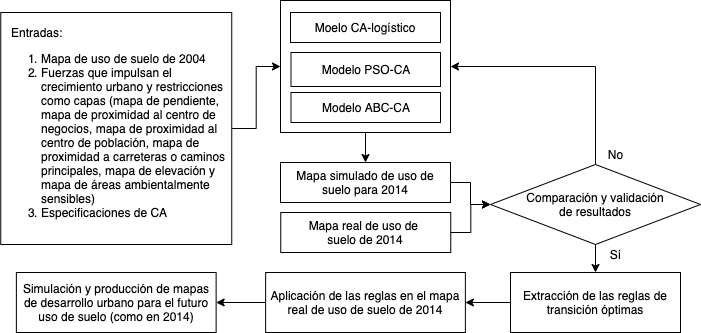
\includegraphics[width=\linewidth]{fig/evaluacion}
	\caption{Modelo de evaluación de los algoritmos.}
	\label{fig:evaluation}
\end{figure}

\begin{figure}[H]
	\centering
	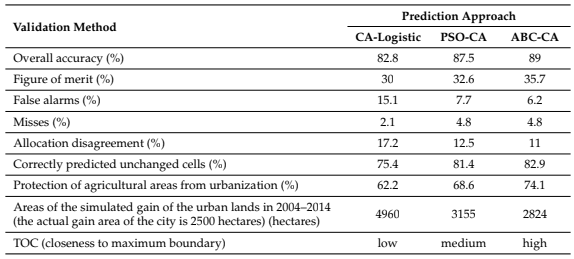
\includegraphics[width=\linewidth]{fig/results}
	\caption{Resultados de la evaluación de los algoritmos. }
	\label{fig:results}
\end{figure}

Como podemos ver en la tabla de resultados, el algoritmo de colonia de abejas fue capaz de obtener un mejor rendimiento en comparación con los otros métodos. Esto ayudará a obtener un mejor despeño en la estimación correcta del crecimiento urbano. Sin embargo, el método aquí planteado sigue teniendo ciertos obstáculos como lo es encontrar una correcta definición de la ecuación que determine al autómata celular.

\section{On Routine Evolution of Complex Cellular Automata}

El aporte principal de este trabajo \citep{bidlo2016routine} es la creación de un método para la obtención de un conjunto de reglas que puedan replicar un comportamiento específico. Sin embargo, es importante resaltar que no se toma en cuenta conocimiento previo del fenómeno que se quiere replicar. Lo que se utiliza es un algoritmo evolutivo, cuya función de aptitud es dependiente del resultado al que se quiere llegar. La codificación de las reglas viene dada de la siguiente forma:

\begin{figure}[H]
	\centering
	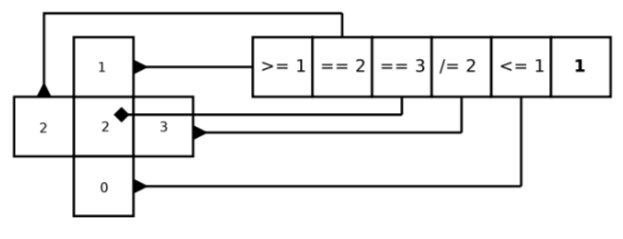
\includegraphics[width=\linewidth]{fig/rulesencoding}
	\caption{Ejemplo de la codificación de las reglas de evolución del autómata con un vecindario de tipo Moore.}
	\label{fig:rulesencoding}
\end{figure}
 % Estado del arte
\chapter{Métodos y metodologías}

En esta sección se detalla cuál fue la metodología empleada para llevar acabo los experimentos. En la figura \ref{fig:metodologia} a continuación, se puede ver el panorama general de dicha metodología experimental.

\begin{figure}[H]
	\centering
	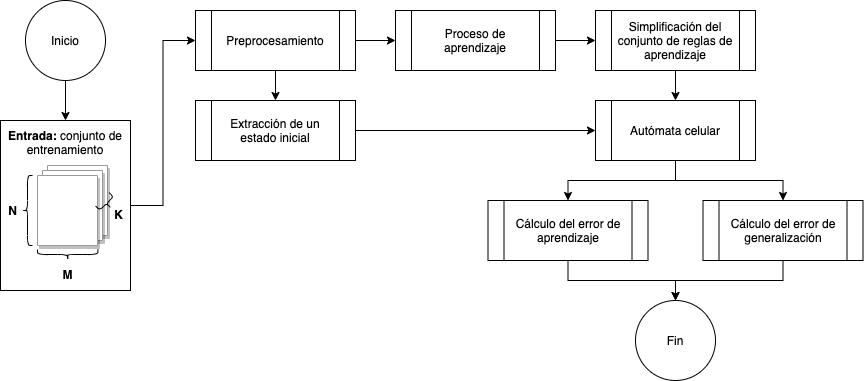
\includegraphics[width=\linewidth]{fig/metodologia}
	\caption{Diagrama general de la metodología.}
	\label{fig:metodologia}
\end{figure}

\section{Conjunto de datos}

Para realizar los experimentos, se optó por adquirir un conjunto de datos que consiste en los estados de la evolución de 4 diferentes autómatas celulares bidimensionales, los cuales fueron obtenidos de \cite{rucker_walker}.
\\
Para cada uno de los autómatas se obtuvieron 200 imágenes de 50x50 pixeles en escala RGB, que se ejemplifican en las imágenes de la Figura \ref{caexamples} a continuación.

\begin{figure}[h]
	
	\begin{subfigure}{0.5\textwidth}
		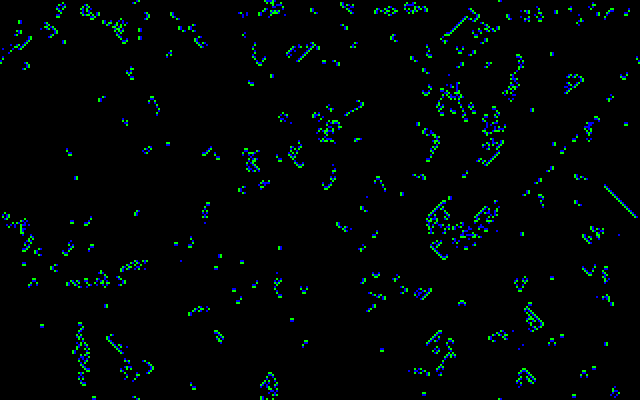
\includegraphics[width=0.9\linewidth, height=5cm]{fig/brain_1} 
		\caption{Brain estado 1}
		\label{fig:brain1}
	\end{subfigure}
	\begin{subfigure}{0.5\textwidth}
		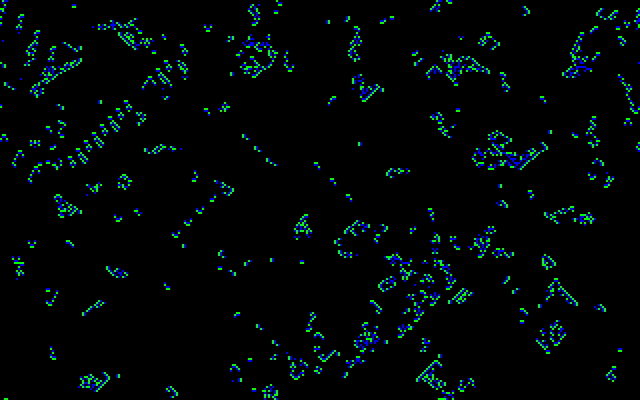
\includegraphics[width=0.9\linewidth, height=5cm]{fig/brain_200}
		\caption{Brain estado 200}
		\label{fig:brain200}
	\end{subfigure}
	\begin{subfigure}{0.5\textwidth}
		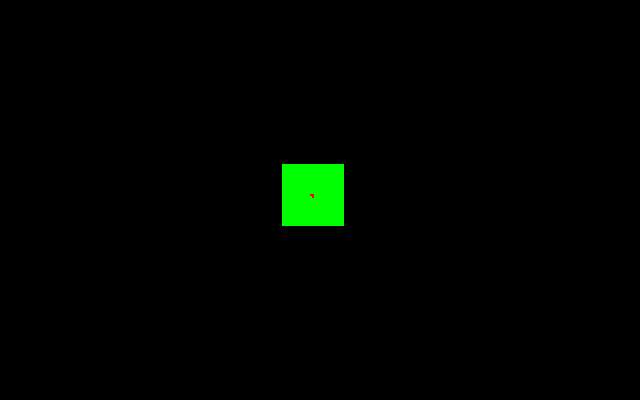
\includegraphics[width=0.9\linewidth, height=5cm]{fig/mite_1}
		\caption{Mite estado 1}
		\label{fig:mite100}
	\end{subfigure}
	\begin{subfigure}{0.5\textwidth}
		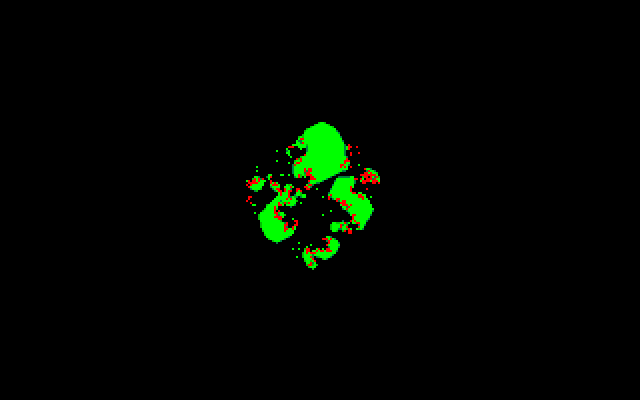
\includegraphics[width=0.9\linewidth, height=5cm]{fig/mite_200}
		\caption{Mite estado 200}
		\label{fig:mite200}
	\end{subfigure}
	
	\caption{Ejemplo del conjunto de datos}
	\label{fig:caexamples}
\end{figure}

A continuación, se mencionan los autómatas celulares en los cuales se implementaron este tipo de imágenes.

\subsection{Brain}

Es un autómata celular bidimensional, desarrollado por Brian Silverman, que consiste en lo siguiente:

\begin{itemize}
	\item \textbf{Vecindario:} es de tipo Moore con 8 vecinos.
	\item \textbf{Espacio de estados:} 3 estados.
	\begin{itemize}
		\item 0 que representa el estado apagado
		\item 1 que representa el estado encendido
		\item 2 que representa el estado muriendo.
	\end{itemize}
	\item \textbf{Función de evolución:} 
	\begin{itemize}
		\item 1 si se encuentra apagado y si dos o mas vecinos se encuentran encendidos.
		\item 2 si en el estado anterior estaba encendido.
		\item 0 si en el estado anterior estaba muriendo.
	\end{itemize}
\end{itemize}

\subsection{Byl}

Es un autómata celular bidimensional, desarrollado por Jhon Byl \citep{BYL1989295}, que consiste en lo siguiente:

\begin{itemize}
	\item \textbf{Vecindario:} es de tipo Von Neumann con 5 vecinos, en el cuadro \ref{tab:bylneigh} podemos ver como se codifica el vecindario.
	\item \textbf{Espacio de estados:} consiste de 6 estados del 0 al 5.
	\item \textbf{Función de evolución:} se muestra en el cuadro \ref{tab:byltransfunction}
\end{itemize}

\begin{table}[H]
	\begin{center}
		\renewcommand{\arraystretch}{1.3}
		\begin{tabular}{ c c c c c}
			\hline
			CTRBL $\rightarrow$ I & CTRBL $\rightarrow$ I & CTRBL $\rightarrow$ I & CTRBL $\rightarrow$ I & CTRBL $\rightarrow$ I \\ 
			\hline
			00003\quad\quad\quad 1& 10003\quad\quad\quad 3 & 20215\quad\quad\quad 5 & 31215\quad\quad\quad 1 & 40242\quad\quad\quad 4 \\  
			00012\quad\quad\quad 2& 10004\quad\quad\quad 0 & 20235\quad\quad\quad 3 & 31223\quad\quad\quad 1 & 40252\quad\quad\quad 0 \\
			00013\quad\quad\quad 1& 10033\quad\quad\quad 0 & 20252\quad\quad\quad 5 & 31233\quad\quad\quad 1 & 40325\quad\quad\quad 5  \\
			00015\quad\quad\quad 2& 10043\quad\quad\quad 1 & 2 - - - - \quad\quad 2 & 31235\quad\quad\quad 5 & 4 - - - - \quad\quad 3  \\
			00025\quad\quad\quad 5& 10321\quad\quad\quad 3 & 30001\quad\quad\quad 0 & 31432\quad\quad\quad 1 & 50022\quad\quad\quad 5 \\
			00031\quad\quad\quad 5& 11253\quad\quad\quad 1 & 30003\quad\quad\quad 0 & 31452\quad\quad\quad 5 & 50032\quad\quad\quad 5  \\
			00032\quad\quad\quad 3& 12453\quad\quad\quad 3 & 30011\quad\quad\quad 0 & 3 - - - - \quad\quad 3 & 50212\quad\quad\quad 4  \\
			00042\quad\quad\quad 2& 1 - - - - \quad\quad 4 & 30012\quad\quad\quad 1 & & 50222\quad\quad\quad 0 \\
			0 - - - - \quad\quad 0 & 20000\quad\quad\quad 0 & 30121\quad\quad\quad 1 & 40003\quad\quad\quad 0 & 50322\quad\quad\quad 0  \\
			& 20015\quad\quad\quad 5 & 30123\quad\quad\quad 1 & 40043\quad\quad\quad 0 & 5 - - - - \quad\quad 2  \\
			10000\quad\quad\quad 0& 20022\quad\quad\quad 0 & 31122\quad\quad\quad 1 & 40212\quad\quad\quad 0 & \\
			10001\quad\quad\quad 0& 20202\quad\quad\quad 0 & 31123\quad\quad\quad 1 & 40232\quad\quad\quad 0 &
		\end{tabular}
		\caption{\label{tab:byltransfunction} Función de evolución de Byl CA \citep{BYL1989295}.}
	\end{center}
\end{table}

\begin{table}[H]
	\begin{center}
		\begin{tabular}{ c c c}
			&T&\\
			L&C&R $\rightarrow$ I\\
			&B&\\
		\end{tabular}
	\end{center}
	\caption{\label{tab:bylneigh} Codificación del vecindario.}
\end{table}

\subsection{Evoloops}
Es un autómata bidimensional, desarrollado por Hiroki Sayama \citep{Sayama1998ConstructingES}, que consiste en lo siguiente:
\begin{itemize}
	\item \textbf{Vecindario:} es de tipo Von Neumann con 5 vecinos, en el cuadro \ref{tab:bylneigh} podemos ver como se codifica el vecindario.
	\item \textbf{Espacio de estados:} consiste de 8 estados del 0 al 7.
	\item \textbf{Función de evolución:} se muestra en el cuadro \ref{tab:evoloopstransfunction}
\end{itemize}

\begin{table}[H]
	\begin{center}
		\renewcommand{\arraystretch}{1.2}
		\resizebox{\textwidth}{!}{%
			\begin{tabular}{ c c c c c c}
				\hline
				CTRBL $\rightarrow$ I & CTRBL $\rightarrow$ I & CTRBL $\rightarrow$ I & CTRBL $\rightarrow$ I & CTRBL $\rightarrow$ I & CTRBL $\rightarrow$ I \\ 
				\hline
				00001\quad\quad\quad2& 10202\quad\quad\quad1& 11272\quad\quad\quad7& 20172\quad\quad\quad2& 21322\quad\quad\quad2& 40125\quad\quad\quad0\\
				00004\quad\quad\quad3& 10211\quad\quad\quad1& 11273\quad\quad\quad5& 20202\quad\quad\quad2& 21422\quad\quad\quad2& 40162\quad\quad\quad0\\
				00012\quad\quad\quad2& 10212\quad\quad\quad1& 11322\quad\quad\quad1& 20203\quad\quad\quad2& 21622\quad\quad\quad2& 40212\quad\quad\quad0\\
				00015\quad\quad\quad2& 10213\quad\quad\quad1& 11332\quad\quad\quad1& 20205\quad\quad\quad2& 21722\quad\quad\quad2& 40215\quad\quad\quad0\\
				00021\quad\quad\quad2& 10221\quad\quad\quad1& 11542\quad\quad\quad4& 20206\quad\quad\quad5& 22224\quad\quad\quad2& 40222\quad\quad\quad1\\
				00024\quad\quad\quad2& 10224\quad\quad\quad4& 11572\quad\quad\quad7& 20207\quad\quad\quad3& 22227\quad\quad\quad2& 40232\quad\quad\quad1\\
				00042\quad\quad\quad2& 10227\quad\quad\quad7& 11624\quad\quad\quad4& 20212\quad\quad\quad2& 22234\quad\quad\quad2& 40262\quad\quad\quad6\\
				00045\quad\quad\quad2& 10232\quad\quad\quad4& 11627\quad\quad\quad7& 20215\quad\quad\quad2& 22237\quad\quad\quad2& 40312\quad\quad\quad0\\
				00075\quad\quad\quad2& 10241\quad\quad\quad4& 12224\quad\quad\quad4& 20221\quad\quad\quad2& 22243\quad\quad\quad2& 40322\quad\quad\quad1\\
				00102\quad\quad\quad2& 10242\quad\quad\quad4& 12227\quad\quad\quad7& 20222\quad\quad\quad2& 22244\quad\quad\quad2& 50002\quad\quad\quad5\\
				00214\quad\quad\quad1& 10243\quad\quad\quad4& 12243\quad\quad\quad4& 20223\quad\quad\quad2& 22273\quad\quad\quad2& 50012\quad\quad\quad5\\
				00217\quad\quad\quad1& 10251\quad\quad\quad1& 12273\quad\quad\quad7& 20232\quad\quad\quad3& 22277\quad\quad\quad2& 50021\quad\quad\quad5\\
				00232\quad\quad\quad2& 10252\quad\quad\quad7& 12324\quad\quad\quad4& 20242\quad\quad\quad2& 22324\quad\quad\quad3& 50023\quad\quad\quad2\\
				01122\quad\quad\quad1& 10254\quad\quad\quad3& 12327\quad\quad\quad7& 20245\quad\quad\quad2& 22327\quad\quad\quad3& 50024\quad\quad\quad5\\
				01212\quad\quad\quad1& 10257\quad\quad\quad7& 12426\quad\quad\quad6& 20252\quad\quad\quad5& 30001\quad\quad\quad3& 50027\quad\quad\quad5\\
				01232\quad\quad\quad1& 10271\quad\quad\quad7& 12433\quad\quad\quad3& 20262\quad\quad\quad0& 30002\quad\quad\quad2& 50042\quad\quad\quad5\\
				01242\quad\quad\quad1& 10272\quad\quad\quad7& 12627\quad\quad\quad6& 20265\quad\quad\quad0& 30003\quad\quad\quad2& 50072\quad\quad\quad5\\
				01245\quad\quad\quad1& 10273\quad\quad\quad5& 20001\quad\quad\quad2& 20272\quad\quad\quad2& 30004\quad\quad\quad3& 50202\quad\quad\quad2\\
				01252\quad\quad\quad6& 10512\quad\quad\quad1& 20002\quad\quad\quad2& 20275\quad\quad\quad2& 30007\quad\quad\quad4& 50205\quad\quad\quad2\\
				01262\quad\quad\quad6& 10542\quad\quad\quad4& 20004\quad\quad\quad2& 20312\quad\quad\quad2& 30012\quad\quad\quad3& 50212\quad\quad\quad5\\
				
		\end{tabular}}
	\end{center}
\end{table}
\begin{table}[H]
	\begin{center}
		\renewcommand{\arraystretch}{1.2}
		\resizebox{\textwidth}{!}{%
			\begin{tabular}{ c c c c c c}
				01272\quad\quad\quad1& 10572\quad\quad\quad7& 20005\quad\quad\quad2& 20322\quad\quad\quad2& 30032\quad\quad\quad2& 50215\quad\quad\quad2\\
				01275\quad\quad\quad1& 10621\quad\quad\quad1& 20006\quad\quad\quad0& 20342\quad\quad\quad2& 30042\quad\quad\quad1& 50242\quad\quad\quad5\\
				01342\quad\quad\quad1& 10624\quad\quad\quad4& 20007\quad\quad\quad1& 20345\quad\quad\quad2& 30102\quad\quad\quad1& 50272\quad\quad\quad5\\
				01372\quad\quad\quad1& 10627\quad\quad\quad7& 20012\quad\quad\quad2& 20372\quad\quad\quad2& 30125\quad\quad\quad0& 50312\quad\quad\quad0\\
				01422\quad\quad\quad1& 11112\quad\quad\quad1& 20015\quad\quad\quad2& 20412\quad\quad\quad2& 30212\quad\quad\quad3& 60202\quad\quad\quad2\\
				01425\quad\quad\quad1& 11122\quad\quad\quad1& 20021\quad\quad\quad2& 20422\quad\quad\quad2& 30242\quad\quad\quad3& 60212\quad\quad\quad2\\
				01432\quad\quad\quad1& 11124\quad\quad\quad4& 20022\quad\quad\quad2& 20442\quad\quad\quad2& 30252\quad\quad\quad1& 60222\quad\quad\quad0\\
				01435\quad\quad\quad1& 11125\quad\quad\quad1& 20023\quad\quad\quad2& 20512\quad\quad\quad2& 30272\quad\quad\quad3& 60242\quad\quad\quad2\\
				01442\quad\quad\quad1& 11127\quad\quad\quad7& 20024\quad\quad\quad2& 20542\quad\quad\quad5& 30332\quad\quad\quad1& 60272\quad\quad\quad2\\
				01462\quad\quad\quad1& 11162\quad\quad\quad1& 20026\quad\quad\quad0& 20572\quad\quad\quad5& 31212\quad\quad\quad3& 61222\quad\quad\quad0\\
				01722\quad\quad\quad1& 11212\quad\quad\quad1& 20027\quad\quad\quad2& 20612\quad\quad\quad5& 31242\quad\quad\quad3& 62224\quad\quad\quad0\\
				01725\quad\quad\quad1& 11213\quad\quad\quad1& 20032\quad\quad\quad4& 20621\quad\quad\quad2& 31252\quad\quad\quad1& 62227\quad\quad\quad0\\
				01756\quad\quad\quad1& 11215\quad\quad\quad1& 20042\quad\quad\quad3& 20642\quad\quad\quad5& 31272\quad\quad\quad3& 70102\quad\quad\quad0\\
				01762\quad\quad\quad1& 11222\quad\quad\quad1& 20045\quad\quad\quad2& 20672\quad\quad\quad5& 32424\quad\quad\quad3& 70112\quad\quad\quad0\\
				01772\quad\quad\quad1& 11224\quad\quad\quad4& 20054\quad\quad\quad5& 20712\quad\quad\quad2& 32425\quad\quad\quad1& 70122\quad\quad\quad0\\
				10001\quad\quad\quad1& 11227\quad\quad\quad7& 20057\quad\quad\quad5& 20722\quad\quad\quad2& 32427\quad\quad\quad3& 70125\quad\quad\quad0\\
				10012\quad\quad\quad1& 11232\quad\quad\quad1& 20062\quad\quad\quad0& 20772\quad\quad\quad2& 32527\quad\quad\quad1& 70162\quad\quad\quad0\\
				10021\quad\quad\quad1& 11242\quad\quad\quad4& 20072\quad\quad\quad2& 21122\quad\quad\quad2& 32727\quad\quad\quad3& 70212\quad\quad\quad0\\
				10024\quad\quad\quad4& 11243\quad\quad\quad4& 20075\quad\quad\quad2& 21222\quad\quad\quad2& 40000\quad\quad\quad1& 70215\quad\quad\quad0\\
				10027\quad\quad\quad7& 11252\quad\quad\quad7& 20102\quad\quad\quad2& 21223\quad\quad\quad2& 40002\quad\quad\quad1& 70222\quad\quad\quad1\\
				10121\quad\quad\quad1& 11254\quad\quad\quad3& 20112\quad\quad\quad2& 21224\quad\quad\quad2& 40102\quad\quad\quad0& 70232\quad\quad\quad0\\
				10124\quad\quad\quad4& 11257\quad\quad\quad7& 20122\quad\quad\quad2& 21227\quad\quad\quad2& 40112\quad\quad\quad0& 70262\quad\quad\quad6\\
				10127\quad\quad\quad7& 11262\quad\quad\quad6& 20142\quad\quad\quad2& 21232\quad\quad\quad3& 40122\quad\quad\quad0& 70312\quad\quad\quad0
		\end{tabular}}
		\caption{\label{tab:evoloopstransfunction} Función de evolución de Evoloops CA \citep{Sayama1998ConstructingES} .}
	\end{center}
\end{table}

\subsection{Mite}

Es un autómata bidimensional, desarrollado por Dan Drake, que consiste en lo siguiente:
\begin{itemize}
	\item \textbf{Vecindario:} es de tipo Moore con 8 vecinos.
	\item \textbf{Espacio de estados:} consiste de 3 estados del 0 al 2.
	\item \textbf{Función de evolución:} 
	\begin{itemize}
		\item mover la posición del predador de manera aleatoria dentro de su vecindario local.
		\item si no hay presa en su posición el predador muere.
		\item si hay suficientes presas en su posición se incrementa el número de predadores.
		\item si hay dos presas juntas se incrementa el número de presas.
	\end{itemize}
\end{itemize}

\section{Preprocesamiento}
Una vez adquiridas las secuencias de imágenes de cada autómata celular, se continúa con los procesos de discretización y binarización que se explican en las subsecciones siguientes.

En términos generales, la discretización consta en pasar las imágenes de los canales RGB a valores discretos, mientras que el proceso de binarización solo se realiza para los datos que se van a ingresar al algoritmo RA1. De cualquier manera, se mencionan a continuación algunas características específicas de cada proceso.

\subsection{Discretización}

La implementación de este procedimiento se realizó en el lenguaje Python y se ejemplifica con el siguiente pseudocódigo.

\begin{algorithm}[H] 
	\SetKwInOut{Input}{entrada}
	\SetKwInOut{Output}{salida}
	\Input{La ruta de la carpeta donde se encuentran las imágenes}
	\Output{Un archivo con formato .pkl que contiene las imágenes procesadas.}
	\SetAlgoLined
	diccionario = \{\} ; contador = 0; imágenes=[ ] \tcc*{inicializaciónes}
	\ForEach{$Imagen$ en $carpeta$}{
		\textbf{Paso 1:}$Imagen'=$   Transformar imagen a escala de grises\;
		\tcc{Se considera a la imagen como una matriz de pixeles}
		nuevaImagen = [ ]\;
		\ForEach{fila en Imagen}{
			\tcc{una fila es un arreglo de pixeles}
			nuevaFila = [ ] \;
			\ForEach{pixel en fila}{ 
				\tcc{un pixel corresponde a un valor entre 0 y 255 despues de la transformación}
				\If{pixel no esta en diccionario}{
					\textbf{Paso 2:} diccionarion[pixel] = contador\;
					\textbf{Paso 3:} contador = contador + 1\;
				}
				\textbf{Paso 4:} nuevaFila.agregar(diccionario[pixel])\;
			}
			\textbf{Paso 5:} nuevaImagen.agregar(nuevaFila)\;
		}
		\textbf{Paso 6:} imagenes.agregar(nuevaImagen)\;
	}
	\textbf{Paso 7:} Guardar imágenes en formato .pkl\;
	\caption{Pseudocódigo para la discretización de las imágenes.}
\end{algorithm}

\subsection{Binarización}

Este proceso se realiza solamente para los datos que ingresarán al algoritmo RA1 debido a que este algoritmo solo es capaz de aprender de datos categóricos. El siguiente pseudocódigo ejemplifica este proceso.

\begin{algorithm}[H] 
	\SetKwInOut{Input}{entrada}
	\SetKwInOut{Output}{salida}
	\Input{MEstado: matriz de estado}
	\Output{El estado binarizado}
	\SetAlgoLined
	nuevoEstado = []\;
	\ForEach{fila en MEstado}{
		\textbf{nuevaFila} = []\;
		\ForEach{celda en fila}{
			\textbf{Paso 1:} Encontrar el dominio de la celda\;
			\textbf{Paso 2:} dominio = ordenarAscendente (dominio)\;
			\ForEach{valor en dominio}{
				\eIf{celda < valor}{
					\textbf{Paso 3a:} nuevaFila.agregar(1)\;
				}{
					\textbf{Paso 3b:} nuevaFila.agregar(0)\;
				}
			}
			
		}
		\textbf{Paso 4:} nuevoEstado.agregar(nuevaFila)\;
	}
	
	\caption{Pseudocódigo para la binarización de las imágenes.}
\end{algorithm}

\section{Algoritmos de aprendizaje}
Los algoritmos de aprendizaje utilizados en este trabajo de investigación son los siguientes:
\begin{itemize}
	\item RA1
	\item GA-Nuggets
	\item LRDEA el algoritmo diseñado en este trabajo.
\end{itemize}

Cabe mencionar que, debido a que no se encontraron las implementaciones de los algoritmos RA1 y GA-Nuggets, fue necesario realizarlas en el lenguaje de programación Python.

\subsection{LRDEA (Local Rule Discovery Evolutive Algorithm)}

Nuestra propuesta de solución para el problema, se basa en un algoritmo genético distribuido cuyo funcionamiento combina el principio del algoritmo RA1 ---que equivale a ir generando cláusulas que cubran a los ejemplos positivos y rechace a los ejemplos negativos---, y el principio de un algoritmo genético ---que implica tener recombinación entre un conjunto de individuos para explorar el espacio de búsqueda---.  El algoritmo propuesto maneja una subpoblación por cada uno de los valores en el espacio de estado del autómata celular.

\subsubsection{Representación}

Al igual que el algoritmo GA-Nuggets, la codificación para cada individuo representa una regla de predicción candidata de la forma IF $Ant$ THEN $Cons$, donde $Ant$ es el antecedente de la regla y $Cons$ es el consecuente. El antecedente $Ant$ consiste en una conjunción de condiciones, donde cada condición es un par vecino valor de la forma $n_i = V_i$, donde $n_i$ es el i-ésimo vecino y $V_{i}$ es un conjunto de los posibles valores que puede tener $n_i$ de la forma $\{v_{0},\dots,v_{n}\}$ donde $v$ es un valor dentro del dominio del vecino $n_i$.
\\
El algoritmo solo maneja valores categóricos, por lo que es necesario discretizar los valores. El consecuente $Cons$ consiste en un solo valor en el dominio que puede tomar la celda que se esta evaluando $c$. Se utiliza el valor -1 para indicar que el par vecino valor no va a formar parte de la regla.


\begin{table}[H]
	\begin{center}
		\begin{tabular}{ c c c c}
			$n_1$&$n_2$&$n_3$&\\
			$n_4$&$c$&$n_5$& $\rightarrow$ Cons\\
			$n_6$&$n_7$&$n_8$&\\
		\end{tabular}
	\end{center}
	\caption{\label{tab:lrdeaneigh} Representación del vecindario.}
\end{table}

Finalmente, conviene mostrar una representación de la codificación de un vecindario como el propuesto en el Cuadro \ref{tab:lrdeaneigh}.

\begin{table}[H]
	\begin{center}
		\resizebox{\textwidth}{!}{%
			\begin{tabular}{ |c| c| c| c| c| c| c| c| c| c|}
				\hline
				$n_1 = V_1$&$n_2 =  V_2$&$n_3=  V_3$& $n_4=  V_4$&$c =  V_c$&$n_5 =  V_5$& $n_6 =  V_6$&$n_7 =  V_7$&$n_8 =  V_8$& Cons\\
				\hline
		\end{tabular}}
	\end{center}
	\caption{\label{tab:lredeacod} Representación de la codificación.}
\end{table}

\subsubsection{Función de aptitud}

La función de aptitud propuesta se define por la siguiente ecuación:

\begin{equation}\label{eq:fitness1}
	Fitness(C,E^{+})=\sum_{i=1}^{|E^{+}|} \left(\frac{1}{|C|}\sum_{j=1}^{|C|} Eq(E^{+}_{ij},C_{j}) \right) 
\end{equation}


\begin{equation}\label{eq:fitness2}
Eq(x,y)=
\begin{cases}
\text1 &\qquad if\ x=y \\
\text0 &\qquad otherwise
\end{cases}
\end{equation}

donde:
\begin{itemize}
	\item \(C\) es el cromosoma.
	\item \(|C|\) es la cardinalidad del cromosoma.
	\item \(E^{+}\) es un subconjunto de los ejemplos que pertenece a la clase para la cual se esta evaluando la aptitud del cromosoma.
	\item \(|E^{+}|\) es la cardinalidad de $E^+$.
	\item \(E^{+}_{i,j}\) es un valor en la posición j del elemento en la posicion i de $E^+$.
	\item \(C_{j}\) es el valor del cromosoma en la posición j.
\end{itemize}

\subsubsection{Mecanismo de selección de padres}

Para el mecanismo de selección de padres se eligió la \emph{selección por torneo}, que consiste en lo siguiente:

\begin{algorithm}[H] 
	\SetKwInOut{Input}{entrada}
	\Input{k (la cantidad de individuos participantes en el torneo)}
	\SetAlgoLined
	\textbf{Paso 1:} Escoger k individuos de la población aleatoriamente\;
	\textbf{Paso 2:} Escoger el individuo más apto del torneo con probabilidad p\;
	\textbf{Paso 3:} Escoger el segundo individuo más apto con probabilidad p(1-p) \;
	\textbf{Paso 4:} Escoger el k-esimo individuo más apto con probabilidad $p(1-p)^k$ \;
	\caption{Pseudocódigo de selección por torneo.}
\end{algorithm}

\subsubsection{Cruza}

Para el proceso de cruce se seleccionó el método de \emph{cruce en un punto} y se lleva a cabo de la siguiente manera.
\\
\begin{algorithm}[H] 
	\SetKwInOut{Input}{entrada}
	\Input{padre1, padre2}
	\SetAlgoLined
	\textbf{Paso 1:} Escoger de forma aleatoria el punto p donde p es menor a la cardinalidad de padre1 y padre2\;
	\textbf{Paso 2:} Partir el cromosoma del padre1 y el padre2 en el punto p\;
	\textbf{Paso 3:} Recombinar la primera mitad del padre1 con la segunda mitad del padre2 para generar al hijo1\;
	\textbf{Paso 4:} Recombinar la segunda mitad del padre1 con la primera mitad del padre2 para generar al hijo2\;
	\caption{Pseudocódigo de cruce en un punto.}
\end{algorithm}

\subsubsection{Mutación}

El operador de mutación consiste en dos partes, la primera es la probabilidad de realizar la mutación o no, y la segunda es la selección del gen que se va a mutar.
\\
Finalmente, el gen mutado puede adquirir un nuevo valor en el conjunto de valores o puede removerse uno de estos valores.

\subsubsection{Mecanismo de selección de sobrevivientes}

Para el mecanismo de selección de sobrevivientes es necesario ordenar los individuos de cada subpoblación y se dividen en dos; se procede a tomar los primeros $n$ elementos de cada una de las mitades, y se descarta el resto.

\section{Simplificación de reglas}

El proceso de simplificación de reglas se divide en dos partes:
\begin{enumerate}
	\item remover redundancia en las cláusulas.
	\item emplear el algoritmo Quine–McCluskey para minimizar las cláusulas.
\end{enumerate}

El primer método de simplificación sirve para eliminar términos que no aportan aportan nueva información, esto es por que otros términos contienen a estos. En el siguiente ejemplo podemos ver como es este proceso.

\begin{figure}[H]
	\centering
	\includegraphics[width=\linewidth]{fig/clausulas}
	\caption{Proceso de simplificación 1.}
	\label{fig:simp1}
\end{figure}

En el diagrama de la figura \ref{fig:simp1} vemos cómo, en la cláusula \emph{a}, los términos 1 y 2 pueden ser reducidos a los términos 4 y 5 de la cláusula \emph{b}, respectivamente. Asimismo, podemos ver cómo el término 3 de \emph{a} no se puede reducir, por lo que pasa a \emph{b} directamente.
\\
\\
Para la simplificación 2 de las reglas se utiliza el algoritmo desarrollado por Willard V.Quine 1955 y extendido Edward J. McCluskey en 1956. Este mecanismo solo se emplea para la simplificación de las reglas generadas por el algoritmo RA1.

\section{Evaluación}

En el proceso de evaluación se emplea la validación \emph{camina hacia adelante} o \emph{Walk-Fordward}, que se ejemplifica en el Algoritmo \ref{walkforward}.

\begin{algorithm}[H] 
	\SetAlgoLined
	\tcc{el rango va del 80\% del total de datos al 100\%}
	\ForEach{i en rango(160,200) }{
		\tcc{tomamos un subconjunto del conjunto de datos}
		\textbf{Paso 1:} entrenamiento = datos[0:(i-1)]\; 
		\tcc{tomamos un elemento adicional del conjunto de datos}
		\textbf{Paso 2:} testing = datos[i] \;
		\tcc{aprendemos del conjunto de entrenamiento}
		\textbf{Paso 3:} aprender(entrenamiento)\;
		\textbf{Paso 4:} vExactitud = exactitud(entrenamiento[i-1])\;
		\textbf{Paso 5:} tExactitud = exactitud(testing)\;
	}
	\caption{Pseudocódigo de validación camina hacia adelante (Walk-Fordward).} \label{walkforward}
\end{algorithm}

La toma de los subconjuntos de datos se representa en la Figura \ref{fig:walkforward}, donde podemos observar la dinámica de ''caminar'' hacia adelante.

\begin{figure}[H]
	\centering
	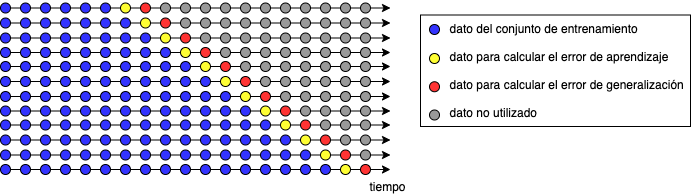
\includegraphics[width=\linewidth]{fig/walkforward}
	\caption{Diagrama de evaluación camina hacia adelante (Walk-Fordward) obtenida de \cite{hyndman2018forecasting}.}
	\label{fig:walkforward}
\end{figure}

Por último, como métrica de desempeño del autómata propuesto, se emplea la \emph{exactitud} (ecuación \ref{eq:exactitud}) para calcular el error de aprendizaje y el error de generalización.

\begin{equation} \label{eq:exactitud}
exactitud = \frac{VP + VN}{VP+FP+VN+FN} 
\end{equation}

donde:
\begin{itemize}
	\item $VP:$ verdaderos positivos.
	\item $VN:$ verdaderos negativos.
	\item $FP:$ falsos positivos.
	\item $FN:$ falsos negativos. 
\end{itemize}


\nomenclature{VP}{Verdaderos Positivos}
\nomenclature{VN}{Verdaderos Negativos}
\nomenclature{FP}{Falsos Positivos}
\nomenclature{FN}{Falsos Negativos}
\nomenclature{LRDEA}{Local Rule Discovery Evolutive Algorithm}
\nomenclature{RGB}{Red Green Blue} % Metodos y metodologia
\chapter{Resultados y análisis}

 % Resultados y analisis
\chapter{Conclusiones y trabajo futuro}

Con la realización de este trabajo de investigación, se diseñó e implementó el nuevo algoritmo de aprendizaje sub-simbólico LRDEA (Local Rule Discovery Evolutive Algorithm), que es capaz de aprender un conjunto de reglas de la forma IF $Ant$ THEN $Cons$, y estas reglas son capaces de reproducir ciertos fenómenos aprendidos.
\\

De igual manera, se seleccionaron e implementaron los algoritmos de aprendizaje de reglas (RA1 y GA-Nuggets) que fueron parcialmente la base del algoritmo propuesto (LRDEA), esto se debe a que cada algoritmo tiene un funcionamiento diferente y, consigo, un comportamiento también diferente.
\\

Se diseñó un modelo de autómata celular con el fin de evaluar los conjuntos de reglas de aprendizaje que se obtuvieron con los algoritmos RA1, GA-Nuggets y LRDEA.
\\

Adicionalmente, se diseñaron procedimientos específicos para la simplificación de los conjuntos de reglas, tal es el caso del proceso que se ejemplifica en la figura \ref{fig:simp1}. Este método elimina la redundancia de las reglas, mientras que el algoritmo Quine-McCluskey colabora en la simplificación de reglas al minimizar las cláusulas generadas por el algoritmo RA1.
\\

Se seleccionaron también los autómatas celulares que reproducen ciertos fenómenos (simulación de la actividad cerebral, el sistema presa-depredador y la autoreplicación) con el fin de obtener datos bidimensionales para ingresarlos a los algoritmos de aprendizaje de reglas y poder compararlos entre sí.
\\

Además, se implementó el algoritmo de evaluación camina hacia adelante, con el cual se lograron obtener los errores de aprendizaje y generalización para cada experimento realizado.
\\

Con base en los resultados de los experimentos realizados, se puede concluir que el algoritmo LRDEA es capaz de aprender un fenómeno a partir de un cierto conjunto de datos proporcionado. Este aprendizaje se realizó con un porcentaje de exactitud que sobrepasa al algoritmo GA-Nuggets en todos los casos. Sin embargo, como se puede observar en las figuras \ref{fig:lrdeabrain}, \ref{fig:lrdeabyl}, \ref{fig:lrdeaevoloops} y \ref{fig:lrdeamite}, es evidente que todavía es posible mejorar la propuesta.
\\

Este espacio de mejora se observa principalmente en que el algoritmo LRDEA puede llegar a tener variaciones muy grandes entre la exactitud dentro del conjunto del entrenamiento y fuera de entrenamiento, en comparación con el algoritmo RA1, que se caracteriza por tener un comportamiento más estable, al menos en los experimentos realizados.
\\

Otra conclusión que es  importante resaltar es que los algoritmos genéticos mutli-poblacionales, como el LRDEA, realizan búsquedas robustas en espacios complejos y, como en este caso se realizó una búsqueda de reglas de aprendizaje a partir de un conjunto de lattices bidimensionales, esta complejidad se incrementa. A pesar de esto, el algoritmo propuesto realiza la búsqueda de reglas de una manera eficiente, lo cual posiciona al LRDEA como un algoritmo genético competitivo en esta tarea, al menos en exactitud, en comparación con el GA-Nuggets y el RA1.

\section{Trabajo a futuro}

Como trabajo a futuro próximo, se propone realizar la experimentación utilizando otros conjuntos de datos, como por ejemplo: imágenes aéreas de áreas urbanas para el aprendizaje de reglas que simulen el crecimiento de población u otros conjuntos de datos cuya representación de estados sea un conjunto de lattices bidimensionales.
\\

De igual manera, se propone investigar una función de aptitud diferente, con la cual sea posible a reducir la variación entre la exactitud dentro y fuera de entrenamiento.
\\

Finalmente, se propone la implementación de otras métricas de evaluación que incluyan tomar en cuenta el tiempo de cómputo que cada algoritmo tomó para llevar a cabo estos u otros experimentos, o bien, diversos métodos de evaluación estadística. % Conclusiones y trabajo futuro
\printnomenclature
%
\bibliographystyle{apalike}
\bibliography{Referencias} 
%% + + + + + + + + + + + + + + + + + + + + + + + + + + + + + + + + + +
% + + + + + + + + + + + + + + + + + + + + + + + + + + + + + + + + + +
%  ____    _   _       _   _                                   __   _
% | __ )  (_) | |__   | | (_)   ___     __ _   _ __    __ _   / _| (_)   __ _
% |  _ \  | | | '_ \  | | | |  / _ \   / _` | | '__|  / _` | | |_  | |  / _` |
% | |_) | | | | |_) | | | | | | (_) | | (_| | | |    | (_| | |  _| | | | (_| |
% |____/  |_| |_.__/  |_| |_|  \___/   \__, | |_|     \__,_| |_|   |_|  \__,_|
%                                      |___/
%
% + + + + + + + + + + + + + + + + + + + + + + + + + + + + + + + + + +
% + + + + + + + + + + + + + + + + + + + + + + + + + + + + + + + + + +
%
% Embedded computing, A VLIM Approach to Architecture, compilers and Tools. Joseph A. Fisher, Paolo Faraboschi, Cliff Young, 2005, by Elsevier Inc. Morgan Kaufmann Publishers. isbn: 1-55860-766-8, printed in USA.
% - - - - - - - - - - - - - - - - - - - - - - - - - - - - - - - - - -
\cleardoublepage
\pagebreak
\addcontentsline{toc}{chapter}{Bibliograf\'{i}a}
\begin{thebibliography}{99}
% - - - - - - - - - - - - - - - - - - - - - - - - - - - - - - - - - -
% - - - - - - - - - - - - - - - - - - - - - - - - - - - - - - - - - -
\bibitem{aylor96}
%Autor:
Aylor, James H. \textsl{et al}. 
%  Año de publicación:
  1996.
% Título de la publicación:
  \emph{The codesign of embedded systems: a unified hardware/software representation}
%%%    [Co-diseño de sistemas empotrados: una representación unificada de hardware/software].
% Edición:
  Primera edición.
% Editorial:
  Kluwer Academic Publishers.
% Lugar de publicación:
  AH Dordrecht. The Netherlands.
% Otros:
  \texttt{ISBN~0-7923-9636-7}.
  Capítulo~2. Páginas 11 y 12.
% * * * * * * * * * * * * * *

\bibitem{godson_processor}
%Autor:
Weiwu Hu. \textsl{et al}. 
%  Año de publicación:
  4 de Mayo del 2006.
% Título de la publicación:
  \emph{Microarchitecture and Performance Analysis of Godson-2 SMT Processor.}
% Edición:
%  Primera edición.
% Editorial:
  IEEE.
% Lugar de publicación:
  %
  \url{http://www.cecs.uci.edu/~papers/iccd2006/papers/paper_38.pdf}
% Otros:
  %\texttt{ISBN?}.
  %Capítulo~2. Páginas 11 y 12.
% * * * * * * * * * * * * * *

\bibitem{MDE93}
%Autor:
 Christopher Mims.
% Año de publicación:
  22 de Octubre de 2010.
% Título de la publicación:
  \emph{Chinese Chip Closes in on Intel, AMD.}
% Edición:
  Technology Review.
% Editorial:
  ACM.
% Lugar de publicación:
  %
  \url{http://technews.acm.org/archives.cfm?searchterm=godson&fo=2010-10-oct/oct-22-2010.html}
% Otros:
% * * * * * * * * * * * * * *


\end{thebibliography}

\appendix
%\cleardoublepage
\pagestyle{plain}
%\tiny{Página en blanco dejada intencionalmente}
\addcontentsline{toc}{chapter}{Apéndices}

% * * * * * * * * * * * * * * * * * * * * * * * * * * * * * * * * * *
\chapter{Tarjeta ML507}
Los elementos de la tarjeta de desarrollo ML507 que fueron utilizados en la implementación del S.E. se listan a continuación.


\begin{itemize}
  \item FPGA XC5VFX70T
	\begin{itemize}
	\item PowerPC 440
	\item 11,200 Slices
	\end{itemize}
  \item DDR2 SODIMM (256 MB)
  \item ZBT SRAM (1 MB)
  \item GTX transceivers
	\begin{itemize}
	\item GTX: SFP (1000Base-X)
	\item GTX: SMA (RX and TX differential pairs)
	\item GTX: SGMII
	\item GTX: PCIe™
	\item GTX: SATA (dual host connections)
	\item GTX clock synthesis chips
	\end{itemize}
  \item Header for second serial port
  \item Soft touch port
\end{itemize}


% \section{FPGA}
% El FPGA que contiene la tarjeta de desarrollo es\ldots
% 
% \section{Paralell Sttrata Flash}
% La memoria flash\ldots

% * * * * * * * * * * * * * * * * * * * * * * * * * * * * * * * * * *


\end{document}
